%definira klasu dokumenta 
\documentclass[12pt]{report} 

%prostor izmedu naredbi \documentclass i \begin{document} se zove uvod. U njemu se nalaze naredbe koje se odnose na cijeli dokument

%osnovni LaTex ne može riješiti sve probleme, pa se koriste različiti paketi koji olakšavaju izradu željenog dokumenta
\usepackage[croatian]{babel} 
\usepackage{amssymb}
\usepackage{amsmath}
\usepackage{txfonts}
\usepackage{mathdots}
\usepackage{titlesec}
\usepackage{array}
\usepackage{lastpage}
\usepackage{etoolbox}
\usepackage{tabularray}
\usepackage{color, colortbl}
\usepackage{adjustbox}
\usepackage{geometry}
\usepackage[classicReIm]{kpfonts}
\usepackage{hyperref}
\usepackage{fancyhdr}

\usepackage{float}
\usepackage{setspace}
\restylefloat{table}


\patchcmd{\chapter}{\thispagestyle{plain}}{\thispagestyle{fancy}}{}{} %redefiniranje stila stranice u paketu fancyhdr

%oblik naslova poglavlja
\titleformat{\chapter}{\normalfont\huge\bfseries}{\thechapter.}{20pt}{\Huge}
\titlespacing{\chapter}{0pt}{0pt}{40pt}


\linespread{1.3} %razmak između redaka

\geometry{a4paper, left=1in, top=1in,}  %oblik stranice

\hypersetup{ colorlinks, citecolor=black, filecolor=black, linkcolor=black,	urlcolor=black }   %izgled poveznice


%prored smanjen između redaka u nabrajanjima i popisima
\newenvironment{packed_enum}{
	\begin{enumerate}
		\setlength{\itemsep}{0pt}
		\setlength{\parskip}{0pt}
		\setlength{\parsep}{0pt}
	}{\end{enumerate}}

\newenvironment{packed_item}{
	\begin{itemize}
		\setlength{\itemsep}{0pt}
		\setlength{\parskip}{0pt}
		\setlength{\parsep}{0pt}
	}{\end{itemize}}




%boja za privatni i udaljeni kljuc u tablicama
\definecolor{LightBlue}{rgb}{0.9,0.9,1}
\definecolor{LightGreen}{rgb}{0.9,1,0.9}

%Promjena teksta za dugačke tablice
\DefTblrTemplate{contfoot-text}{normal}{Nastavljeno na idućoj stranici}
\SetTblrTemplate{contfoot-text}{normal}
\DefTblrTemplate{conthead-text}{normal}{(Nastavljeno)}
\SetTblrTemplate{conthead-text}{normal}
\DefTblrTemplate{middlehead,lasthead}{normal}{Nastavljeno od prethodne stranice}
\SetTblrTemplate{middlehead,lasthead}{normal}

%podesavanje zaglavlja i podnožja

\pagestyle{fancy}
\lhead{Programsko inženjerstvo}
\rhead{$<$Projektni zadatak$>$}
\lfoot{$<$Naziv grupe$>$}
\cfoot{stranica \thepage/\pageref{LastPage}}
\rfoot{\today}
\renewcommand{\headrulewidth}{0.2pt}
\renewcommand{\footrulewidth}{0.2pt}


\begin{document} 
	
	
	
	\begin{titlepage}
		\begin{center}
			\vspace*{\stretch{1.0}} %u kombinaciji s ostalim \vspace naredbama definira razmak između redaka teksta
			\LARGE Programsko inženjerstvo\\
			\large Ak. god. 2023./2024.\\
			
			\vspace*{\stretch{3.0}}
			
			\huge $<$WildTrack$>$\\
			\Large Dokumentacija, Rev. 1\textit{$<$1 ili 2$>$}\\
			
			\vspace*{\stretch{12.0}}
			\normalsize
			Grupa: \textit{$<$LovciNa$>$}\\
			Voditelj: \textit{$ $Mia Sara Matušin$ $}\\
			
			
			\vspace*{\stretch{1.0}}
			Datum predaje: \textit{$<$dan$>$. $<$mjesec$>$. $<$godina$>$.}\\
	
			\vspace*{\stretch{4.0}}
			
			Nastavnik: \textit{$<$Ime i prezime nastavnika zaduženog za vašu grupu$>$}\\
		
		\end{center}

	
	\end{titlepage}

	
	\tableofcontents


	\chapter{Dnevnik promjena dokumentacije}
		
		\textbf{\textit{Kontinuirano osvježavanje}}\\
				
		
		\begin{longtblr}[
				label=none
			]{
				width = \textwidth, 
				colspec={|X[2]|X[13]|X[3]|X[3]|}, 
				rowhead = 1
			}
			\hline
			\textbf{Rev.}	& \textbf{Opis promjene/dodatka} & \textbf{Autori} & \textbf{Datum}\\[3pt] \hline
			0.1 & Napravljen predložak.	& Mia Sara Matušin & 22.10.2023. 		\\[3pt] \hline 
			0.2	& Dodani funkcionalni zahtjevi. & Nikola Jamić & 23.10.2023. 	\\[3pt] \hline 
			0.3 & Dodana prva verzija obrazaca uporabe. & Gabriela Oroz, Lana Barišić & 23.10.2023. \\[3pt] \hline 
			0.4 & Dodan prvi dio opisa projektnog zadatka & Mia Sara Matušin & 23.10.2023. \\[3pt] \hline 
			0.8 & Povijest rada i trenutni status implementacije,\newline Zaključci i plan daljnjeg rada & * & 28.08.2013. \\[3pt] \hline 
			0.9 & Opisi obrazaca uporabe & * & 07.09.2013. \\[3pt] \hline 
			0.10 & Preveden uvod & * & 08.09.2013. \\[3pt] \hline 
			0.11 & Sekvencijski dijagrami & * & 09.09.2013. \\[3pt] \hline 
			0.12.1 & Započeo dijagrame razreda & * & 10.09.2013. \\[3pt] \hline 
			0.12.2 & Nastavak dijagrama razreda & * & 11.09.2013. \\[3pt] \hline 
			\textbf{1.0} & Verzija samo s bitnim dijelovima za 1. ciklus & * & 11.09.2013. \\[3pt] \hline 
			1.1 & Uređivanje teksta -- funkcionalni i nefunkcionalni zahtjevi & * \newline * & 14.09.2013. \\[3pt] \hline 
			1.2 & Manje izmjene:Timer - Brojilo vremena & * & 15.09.2013. \\[3pt] \hline 
			1.3 & Popravljeni dijagrami obrazaca uporabe & * & 15.09.2013. \\[3pt] \hline 
			1.5 & Generalna revizija strukture dokumenta & * & 19.09.2013. \\[3pt] \hline 
			1.5.1 & Manja revizija (dijagram razmještaja) & * & 20.09.2013. \\[3pt] \hline 
			\textbf{2.0} & Konačni tekst predloška dokumentacije  & * & 28.09.2013. \\[3pt] \hline 
			&  &  & \\[3pt] \hline	
		\end{longtblr}
	
	
		\textit{Moraju postojati glavne revizije dokumenata 1.0 i 2.0 na kraju prvog i drugog ciklusa. Između tih revizija mogu postojati manje revizije već prema tome kako se dokument bude nadopunjavao. Očekuje se da nakon svake značajnije promjene (dodatka, izmjene, uklanjanja dijelova teksta i popratnih grafičkih sadržaja) dokumenta se to zabilježi kao revizija. Npr., revizije unutar prvog ciklusa će imati oznake 0.1, 0.2, …, 0.9, 0.10, 0.11.. sve do konačne revizije prvog ciklusa 1.0. U drugom ciklusu se nastavlja s revizijama 1.1, 1.2, itd.}
	\chapter{Opis projektnog zadatka}
		
		\textbf{\textit{dio 1. revizije}}\\
		
		\textit{Na osnovi projektnog zadatka detaljno opisati korisničke zahtjeve. Što jasnije opisati cilj projektnog zadatka, razraditi problematiku zadatka, dodati nove aspekte problema i potencijalnih rješenja. Očekuje se minimalno 3, a poželjno 4-5 stranica opisa.	Teme koje treba dodatno razraditi u ovom poglavlju su:}
		\begin{packed_item}
			\item \textit{potencijalna korist ovog projekta}
			\item \textit{postojeća slična rješenja (istražiti i ukratko opisati razlike u odnosu na zadani zadatak). Dodajte slike koja predočavaju slična rješenja.}
			\item \textit{skup korisnika koji bi mogao biti zainteresiran za ostvareno rješenje.}
			\item \textit{mogućnost prilagodbe rješenja }
			\item \textit{opseg projektnog zadatka}
			\item \textit{moguće nadogradnje projektnog zadatka}
		\end{packed_item}
		
		\textit{Za pomoć pogledati reference navedene u poglavlju „Popis literature“, a po potrebi konzultirati sadržaj na internetu koji nudi dobre smjernice u tom pogledu.}
		\eject
		
		
		Cilj ovog zadatka je napraviti aplikacijsko programsko sučelje koje će olakšati komunikaciju između istraživača, voditelja postaja te tragača u akcijama praćenja divljih životinja.
		
		Prvi korak za korištenje aplikacije je registracija. Prilikom registracije korisnik odabire koju bi ulogu imao u aplikaciji. To može biti istraživač, voditelj postaje ili tragač.
		Podaci koje je potrebno unijeti pri registraciji su sljedeći:
		\begin{packed_item}
			\item \textit{korisničko ime}
			\item \textit{fotografija}
			\item \textit{lozinka}
			\item \textit{ime}
			\item \textit{prezime}
			\item \textit{email adresa.}
		\end{packed_item}
		
		Registracija završava potvrdom preko emaila, te dodatno voditelja i istraživača treba potvrditi administrator. Sličan primjer obrasca za registraciju prikazan je u nastavku na slici 2.1.
		
		\begin{figure}[H]
			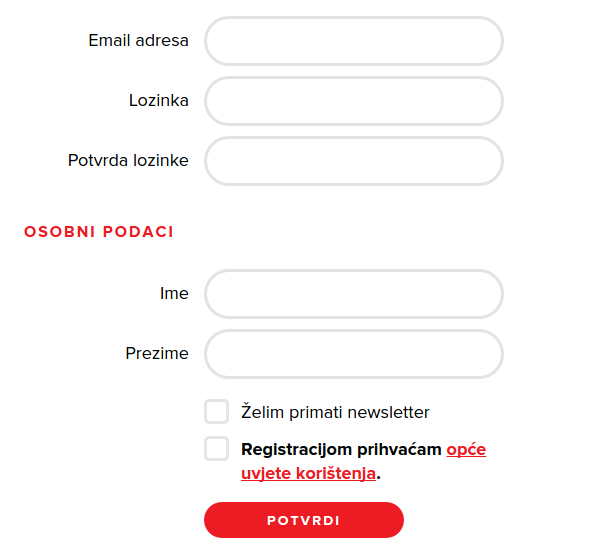
\includegraphics[scale=0.75]{slike/probrazac.PNG} %veličina u odnosu na širinu linije
			\centering
			\caption{Primjer obrasca za registraciju/prijavu}
			\label{fig:probrasca} %label mora biti drugaciji za svaku sliku
		\end{figure}
		
		
		
		\textbf{Voditelj} ima svoju postaju koja ima naziv po području na kojem se nalazi (npr. Kopački rit, Velebit…). Također posjeduje popis \textbf{tragača} koji su dio njegove postaje te na koji način mogu obavljati istraživanje. Mogućnosti kretanja tragača su sljedeće:
		\begin{packed_item}
			\item \textit{pješke}
			\item \textit{automobilom}
			\item \textit{cross motorom}
			\item \textit{brodom}
			\item \textit{dronom}
			\item \textit{helikopterom.}
		\end{packed_item}
		
		Akcija kreće tako što \textbf{istraživač} izda zahtjev za novom akcijom te od voditelja postaje traži da pošalje kvalificirane tragače. Istraživač može preko karte koja mu se prikazuje zadati zadatke svim tragačima na akciji. Tragač se može maknuti s akcije nakon što izvrši sve zadatke koji su mu zadani.
		
		Zadaci su da tragač prođe određenom rutom te dođe do neke lokacije i postavi kameru ili gps uređaj. Na nekoj akciji istraživač i tragač mogu ostaviti komentar na karti.
		
		Cilj svih akcija je pratiti životinje te odrediti povijest njihovog kretanja zbog čega sve životinje imaju gps uređaj. Praćene životinje trebaju imati sljedeće podatke:
		\begin{packed_item}
			\item \textit{naziv vrste}
			\item \textit{slika}
			\item \textit{opis.}
		\end{packed_item}
		
		Sve karte koje se prikazuju su toplinske karte (eng. \textit{heatmaps}). Primjer jedne takve toplinske karte je u nastavku na slici 2.2.
		
		\begin{figure}[H]
			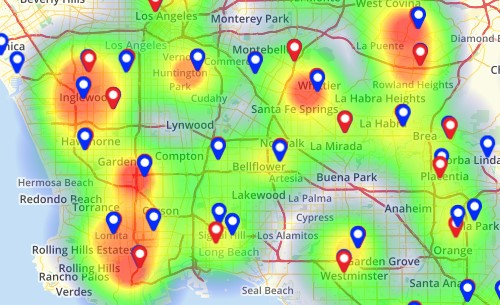
\includegraphics[scale=0.8]{slike/heatmap.JPG} %veličina u odnosu na širinu linije
			\centering
			\caption{Primjer toplinske karte}
			\label{fig:prkarte} %label mora biti drugaciji za svaku sliku
		\end{figure}
		
		Istraživač može izabrati koja će mu se karta prikazati. Može pregledavati karte s podacima o praćenim životinjama:
		\begin{packed_item}
			\item \textit{povijesne pozicije svih praćenih životinja }
			\item \textit{trenutne pozicije svih praćenih životinja.}
		\end{packed_item}
		
		Dodatna stavka koju je potrebno odabrati je želi li podatke o određenoj jedinki ili o svim životinjama neke vrste. 
		Osim toga, ima pristup kartama s podacima o tragačima. Karte koje može pregledavati sadržavaju sljedeće podatke:
		\begin{packed_item}
			\item \textit{povijesne pozicije svih tragača na jednoj akciji}
			\item \textit{trenutne pozicije svih aktivnih tragača na jednoj akciji.}
		\end{packed_item}
		
		Tragače koje želi imati prikazane na karti treba odabrati po tipu prijevoza ili može pregledavati pozicije pojedinačnih tragača.
		
		Također, pristup karti trenutne akcije u kojoj je sudionik ima i tragač.
		Na njegovoj su karti vidljivi sljedeći podaci:
		\begin{packed_item}
			\item \textit{zadaci koje on treba obaviti}
			\item \textit{trenutna pozicija ostalih aktivnih tragača na toj akciji}
			\item \textit{trenutna pozicija praćenih životinja.}
		\end{packed_item}
		
		Pronašli smo nekoliko aplikacija koje imaju sličnu ulogu kao naša te su navedene u nastavku.
		
		Aplikacija \textit{eWildLife} je aplikacija s geooznakama za praćenje divljih životinja, slučajeve ubijanja istih te sukobe čovjeka i životinja te životinja međusobno. U nastavku na slici 2.3. prikazana je stranica za unošenje novih sukoba u ovoj aplikaciji.
		
		\begin{figure}[H]
			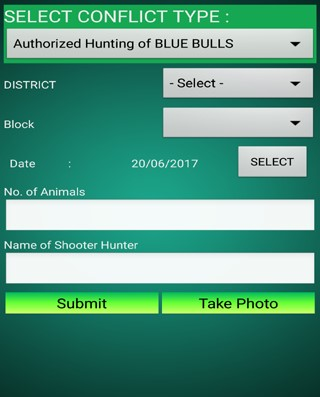
\includegraphics[scale=0.75]{slike/primjera1.JPG} %veličina u odnosu na širinu linije
			\centering
			\caption{Aplikacija eWildLife}
			\label{fig:ewildlife} %label mora biti drugaciji za svaku sliku
		\end{figure}
		
		Aplikacija \textit{Kwibi} bavi se sličnom problematikom kao prethodno navedena aplikacija, rješava probleme sukoba između ljudi i divljih životinja. Ova aplikacija koristi kartu, što je slično kao i u našoj aplikaciji, a njihov je primjer u nastavku na slici 2.4.
		
		\begin{figure}[H]
			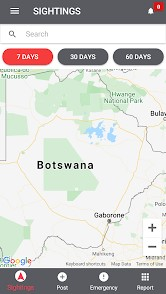
\includegraphics[scale=0.75]{slike/primjera2.JPG} %veličina u odnosu na širinu linije
			\centering
			\caption{Aplikacija Kwibi}
			\label{fig:kwibi} %label mora biti drugaciji za svaku sliku
		\end{figure}
		
		Sljedeća je aplikacija \textit{IMammalia} koja je pokrenuta u sklopu projekta MammalNet diljem Europe, a između ostalog i na Agronomskom fakultetu u Zagrebu. Na stranicu se može registrirati kao tragač ili osmatrač. Tragači u aplikaciju postavljaju fotografije divljih životinja sa svojih kamera koje osmatrači mogu pregledavati i kategorizirati. U nastavku je primjer jedne takve fotografije na slici 2.5.
		
		\begin{figure}[H]
			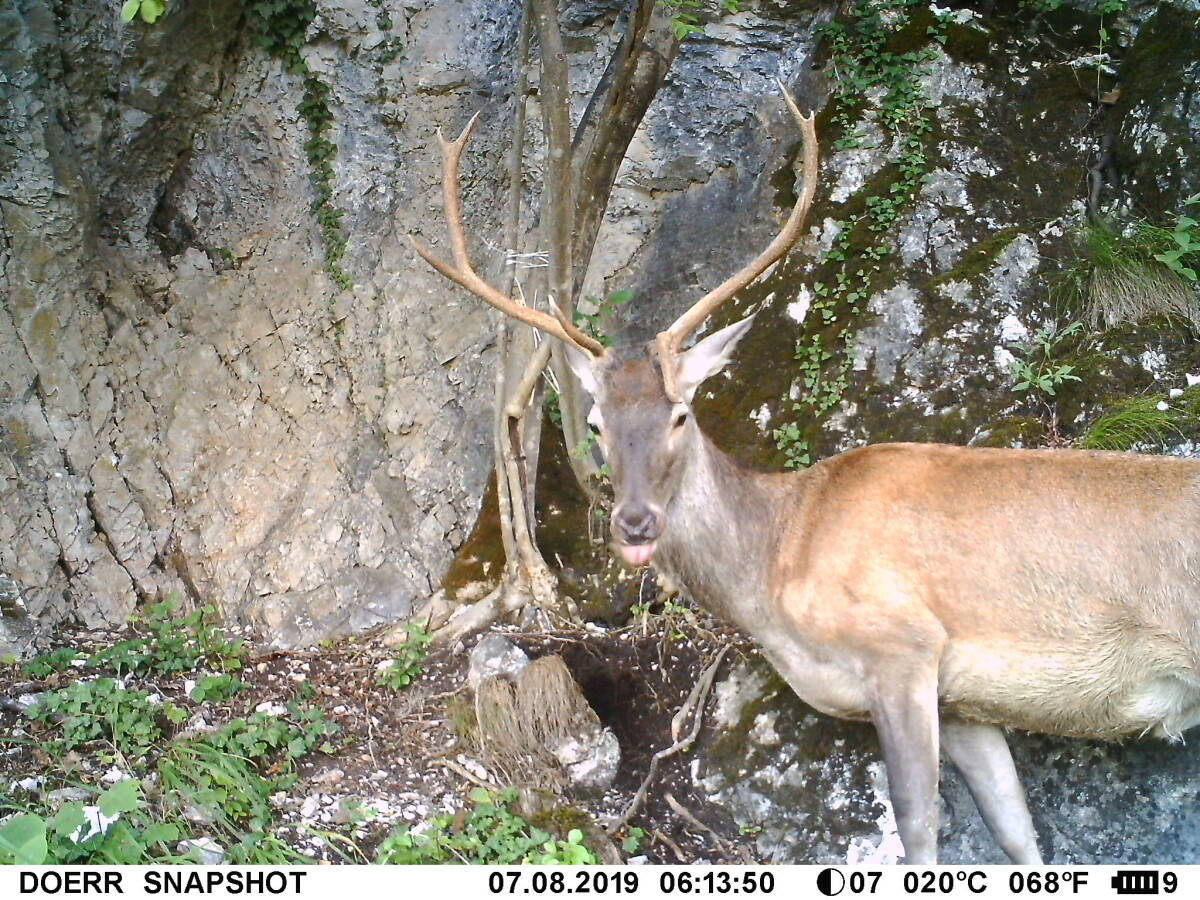
\includegraphics[scale=0.75]{slike/primjera3.JPG} %veličina u odnosu na širinu linije
			\centering
			\caption{Aplikacija IMammalia}
			\label{fig:mammal} %label mora biti drugaciji za svaku sliku
		\end{figure}
		
		Neke od ideja koje je naš tim smislio, a mogle bi u budućnosti unaprijediti aplikaciju kao što je naša su sljedeće:
		\begin{packed_item}
			\item \textit{prikazane male ikonice životinja na karti}
			\item \textit{klikom na životinju otvara se detaljan opis i fotografija vrste}
			\item \textit{svijetli i tamni način rada}
			\item \textit{algoritam za automatsko slanje najkompatibilnijih tragača na akciju, bez posredovanja voditelja postaje.}
		\end{packed_item}
		
		
		\section{Primjeri u \LaTeX u}
		
		\textit{Ovo potpoglavlje izbrisati.}\\

		U nastavku se nalaze različiti primjeri kako koristiti osnovne funkcionalnosti \LaTeX a koje su potrebne za izradu dokumentacije. Za dodatnu pomoć obratiti se asistentu na projektu ili potražiti upute na sljedećim web sjedištima:
		\begin{itemize}
			\item Upute za izradu diplomskog rada u \LaTeX u - \url{https://www.fer.unizg.hr/_download/repository/LaTeX-upute.pdf}
			\item \LaTeX\ projekt - \url{https://www.latex-project.org/help/}
			\item StackExchange za Tex - \url{https://tex.stackexchange.com/}\\
		
		\end{itemize} 	


		
		\noindent \underbar{podcrtani tekst}, \textbf{podebljani tekst}, 	\textit{nagnuti tekst}\\
		\noindent \normalsize primjer \large primjer \Large primjer \LARGE {primjer} \huge {primjer} \Huge primjer \normalsize
				
		\begin{packed_item}
			
			\item  primjer
			\item  primjer
			\item  primjer
			\item[] \begin{packed_enum}
				\item primjer
				\item[] \begin{packed_enum}
					\item[1.a] primjer
					\item[b] primjer
				\end{packed_enum}
				\item primjer
			\end{packed_enum}
			
		\end{packed_item}
		
		\noindent primjer url-a: \url{https://www.fer.unizg.hr/predmet/proinz/projekt}
		
		\noindent posebni znakovi: \# \$ \% \& \{ \} \_ 
		$|$ $<$ $>$ 
		\^{} 
		\~{} 
		$\backslash$ 
		
		
		\begin{longtblr}[
			label=none,
			entry=none
			]{
				width = \textwidth,
				colspec={|X[8,l]|X[8, l]|X[16, l]|}, 
				rowhead = 1,
			} %definicija širine tablice, širine stupaca, poravnanje i broja redaka naslova tablice
			\hline \SetCell[c=3]{c}{\textbf{naslov unutar tablice}}	 \\ \hline[3pt]
			\SetCell{LightGreen}IDKorisnik & INT	&  	Lorem ipsum dolor sit amet, consectetur adipiscing elit, sed do eiusmod  	\\ \hline
			korisnickoIme	& VARCHAR &   	\\ \hline 
			email & VARCHAR &   \\ \hline 
			ime & VARCHAR	&  		\\ \hline 
			\SetCell{LightBlue} primjer	& VARCHAR &   	\\ \hline 
		\end{longtblr}
		

		\begin{longtblr}[
				caption = {Naslov s referencom izvan tablice},
				entry = {Short Caption},
			]{
				width = \textwidth, 
				colspec = {|X[8,l]|X[8,l]|X[16,l]|}, 
				rowhead = 1,
			}
			\hline
			\SetCell{LightGreen}IDKorisnik & INT	&  	Lorem ipsum dolor sit amet, consectetur adipiscing elit, sed do eiusmod  	\\ \hline
			korisnickoIme	& VARCHAR &   	\\ \hline 
			email & VARCHAR &   \\ \hline 
			ime & VARCHAR	&  		\\ \hline 
			\SetCell{LightBlue} primjer	& VARCHAR &   	\\ \hline 
		\end{longtblr}
	


		
		
		%unos slike
		\begin{figure}[H]
			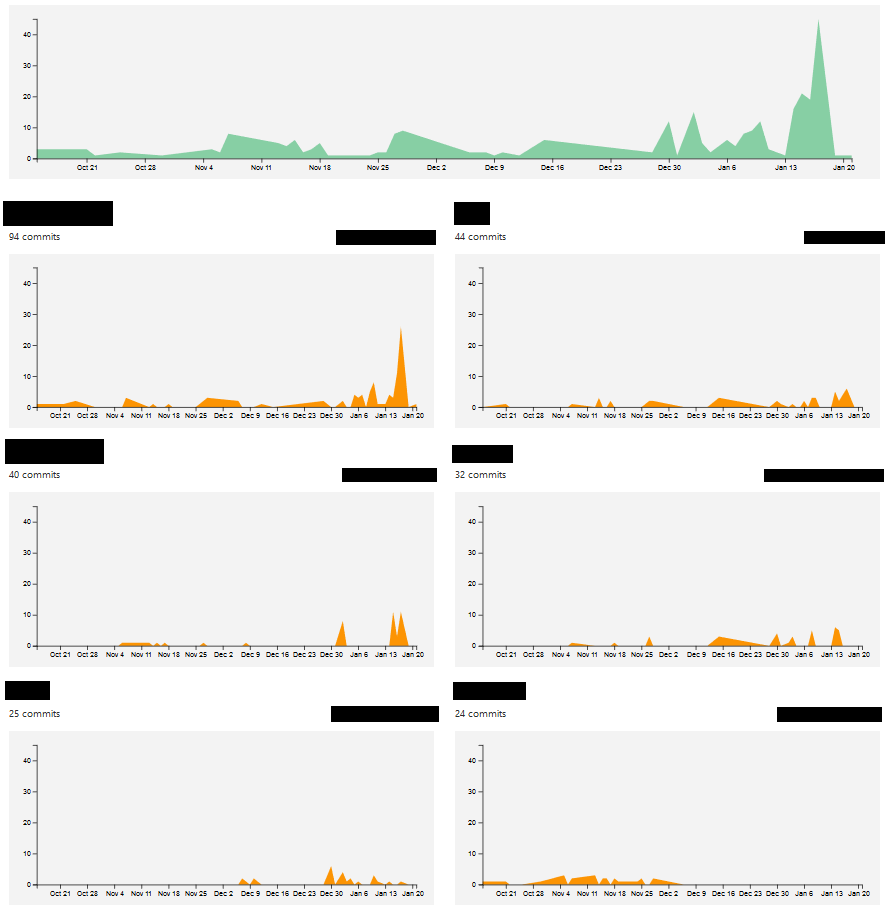
\includegraphics[scale=0.4]{slike/aktivnost.PNG} %veličina slike u odnosu na originalnu datoteku i pozicija slike
			\centering
			\caption{Primjer slike s potpisom}
			\label{fig:promjene}
		\end{figure}
		
		\begin{figure}[H]
			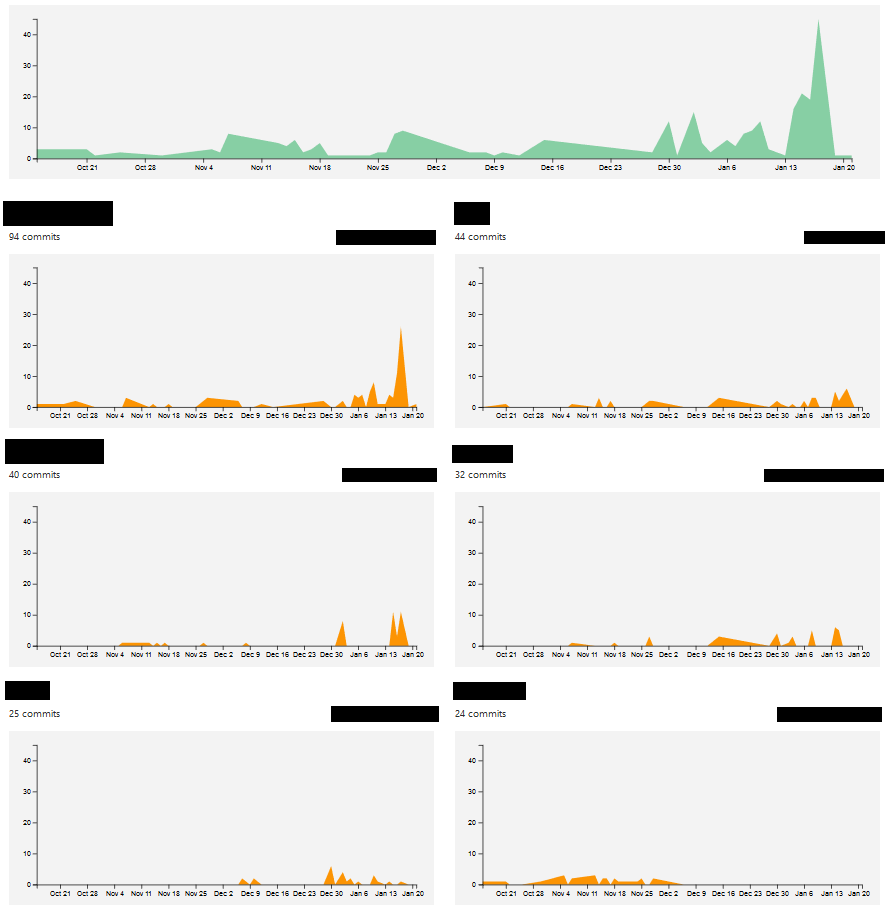
\includegraphics[width=\textwidth]{slike/aktivnost.PNG} %veličina u odnosu na širinu linije
			\caption{Primjer slike s potpisom 2}
			\label{fig:promjene2} %label mora biti drugaciji za svaku sliku
		\end{figure}
		
		Referenciranje slike \ref{fig:promjene2} u tekstu.
		
		\eject
		
	
	\chapter{Specifikacija programske potpore}
		
	\section{Funkcionalni zahtjevi}
			
			\textbf{\textit{dio 1. revizije}}\\
			
			\textit{Navesti \textbf{dionike} koji imaju \textbf{interes u ovom sustavu} ili  \textbf{su nositelji odgovornosti}. To su prije svega korisnici, ali i administratori sustava, naručitelji, razvojni tim.}\\
				
			\textit{Navesti \textbf{aktore} koji izravno \textbf{koriste} ili \textbf{komuniciraju sa sustavom}. Oni mogu imati inicijatorsku ulogu, tj. započinju određene procese u sustavu ili samo sudioničku ulogu, tj. obavljaju određeni posao. Za svakog aktora navesti funkcionalne zahtjeve koji se na njega odnose.}\\
			
			
			\noindent \textbf{Dionici:}
			
			\begin{packed_enum}
				
				\item Vlasnik (naručitelj)
				\item Registrirani korisnici:
							
					\begin{packed_enum}
						\item Voditelji
						\item Istraživači
						\item Tragači
					\end{packed_enum}
					
				\item Razvojni tim
				\item Administrator
				
				
			\end{packed_enum}
			
			\noindent \textbf{Aktori i njihovi funkcionalni zahtjevi:}
			
			
			\begin{packed_enum}
				
				\item  \underbar{Neregistrirani korisnik (sudionik) može:}
				
				\begin{packed_enum}
					
					\item poslati zahtjev za registraciju sa željenom ulogom za koju se prijavljuje (istraživač, voditelj postaje ili tragač na terenu)
				
				\end{packed_enum}
				
				\item \underbar{Istraživač (inicijator) može:}
				
				\begin{packed_enum}
					
					\item stvoriti nove akcije pretraživanja i praćenja
					\item poslati zahtjev voditelju za tragača s potrebnim kvalifikacijama
					\item pojedinačno zadati zadatke tragačima
						\begin{packed_enum}
							\item dati komentar za zadani zadatak
						\end{packed_enum}
					\item pristupiti interaktivnoj karti s informacijama o poziciji tragača, životinja i postaja
						\begin{packed_enum}
							\item ostaviti komentar za ostale sudionike
						\end{packed_enum} 
					\item odabrati način izrade karata (povijesne pozicije životinja, filtrirano po vrsti, filtrirano po jedinki, trenutne pozicije životinja; povijesne pozicije tragača, filitrirano po tipu prijevoza, filtrirano pojedinačno po tragaču, trenutne pozicije tragača)
					
				\end{packed_enum}	
				
				\item \underbar{Voditelj postaje (inicijator) može:}
				
				\begin{packed_enum}
					
					\item definirati tragače njegove postaje
						\begin{packed_enum}
							\item definirati način na koji su osposobljeni izvoditi pretraživanje
						\end{packed_enum}
					\item odabrati konkretne tragače za pojedinu akciju
					
				\end{packed_enum}
			
				\item \underbar{Tragač na terenu (inicijator) može:}
					
					\begin{packed_enum}
						\item biti osposobljen za obavljanje zadataka na različite načine (pješke, dronom, automobilom, 
						cross motorom, brodom, helikopterom)
						\item ostaviti komentar o životinji tijekom akcije
						\item maknuti se s akcije završetkom potrebnih zadataka
						\item pristupiti interaktivnoj karti s informacijama o zadacima, poziciji tragača te trenutnim pozicijama životinja
							\begin{packed_enum}
								\item ostaviti komentar za ostale sudionike
							\end{packed_enum}
					\end{packed_enum}
					
				\item \underbar{Administrator (inicijator) može:}
				
					\begin{packed_enum}
						\item vidjeti popis registriranih korisnika i njihove podatke
						\begin{packed_enum}
							\item mijenjati prava i podatke registriranih korisnika
						\end{packed_enum}
						\item potvrditi istraživača i voditelja postaje
					\end{packed_enum}
					
				\item \underbar{Baza podataka (sudionik):}
				
					\begin{packed_enum}
						\item pohranjuje sve podatke o korisnicima i njihovim ovlastima
						\item pohranjuje sve podatke o postajama i njihovim lokacijama
						\item pohranjuje sve podatke o životinjama i njihovim lokacijama
					\end{packed_enum}
			\end{packed_enum}
			
			
			\eject 
			
			
				
			\subsection{Obrasci uporabe}
				
				\textbf{\textit{dio 1. revizije}}
				
				\subsubsection{Opis obrazaca uporabe}
					\textit{Funkcionalne zahtjeve razraditi u obliku obrazaca uporabe. Svaki obrazac je potrebno razraditi prema donjem predlošku. Ukoliko u nekom koraku može doći do odstupanja, potrebno je to odstupanje opisati i po mogućnosti ponuditi rješenje kojim bi se tijek obrasca vratio na osnovni tijek.}\\
					
					\noindent \underbar{\textbf{UC1 - Registracija}}
					\begin{packed_item}
						
						\item \textbf{Glavni sudionik: }Korisnik
						\item  \textbf{Cilj:} Izrada korisničkog računa za pristup sustavu
						\item  \textbf{Sudionici:} Baza podataka
						\item  \textbf{Preduvjet:} -
						\item  \textbf{Opis osnovnog tijeka:}
						
						\item[] \begin{packed_enum}
							
							\item Odabir opcije registracija
							\item Odabir uloge
							\item Unos osobnih podataka (korisničko ime, fotografija, lozinka, ime, prezime i email adresa)
							\item Slanje zahtjeva za registraciju
							\item Potvrđivanje registracije preko email adrese
						
								\end{packed_enum}
								
						\item  \textbf{Opis mogućih odstupanja:}
						
						\item[] \begin{packed_item}
							
							\item[3.a] Zauzeto korisničko ime
							\begin{packed_enum}
								
								\item Sustav obavještava korisnika da je potrebno upotrijebiti drugo korisničko ime
								
								\end{packed_enum}
							
							\item[3.b] Krivi format lozinke \begin{packed_enum}
								
								\item Sustav obavještava korisnika o uvjetu koji nije zadovoljen da bi lozinka bila ispravna
								
								\end{packed_enum}
							
							\item[3.c] Nepotpuna prijava \begin{packed_enum}
								
								\item Sustav obavještava korisnika o podacima koji mu nedostaju za uspješnu registraciju
								
								\end{packed_enum}
							
							\item[5.a] Nije potvrđena registracije preko email adrese \begin{packed_enum}
								
								\item Sustav obavještava korisnika da mora potvrditi registraciju preko email adrese
								
							\end{packed_enum}
							
						\end{packed_item}
						
					\end{packed_item}
					
					
					\noindent \underbar{\textbf{UC2 - Potvrda registracije od strane administratora}}
					\begin{packed_item}
						
						\item \textbf{Glavni sudionik: }Administrator
						\item  \textbf{Cilj:} Potvrda registracije istraživača i voditelja
						\item  \textbf{Sudionici:} Baza podataka
						\item  \textbf{Preduvjet:} Istraživač ili voditelj je poslao zahtjev za registraciju
						\item  \textbf{Opis osnovnog tijeka:}
						
						\item[] \begin{packed_enum}
							
							\item Odabir opcije potvrđivanja registracije istraživača i voditelja
							
						\end{packed_enum}
						
						\item  \textbf{Opis mogućih odstupanja:}
						
						\item[] \begin{packed_item}
							
							\item[1.a] Administrator ne potvrđuje registraciju istraživača ili voditelja
							\item[] \begin{packed_enum}
								
								\item Sustav obavještava korisnika da mu nije potvrđena registracija i predlaže da sudjeluje kao tragač
								
								\end{packed_enum}
							
						\end{packed_item}
						
					\end{packed_item}
					
					
					\noindent \underbar{\textbf{UC3 - Prijava u sustav}}
					\begin{packed_item}
						
						\item \textbf{Glavni sudionik: }Korisnik
						\item  \textbf{Cilj:} Korištenje aplikacije
						\item  \textbf{Sudionici:} Baza podataka
						\item  \textbf{Preduvjet:} Registracija
						\item  \textbf{Opis osnovnog tijeka:}
						
						\item[] \begin{packed_enum}
							
							\item Odabir opcije prijava
							\item Unos podataka (korisničko ime i lozinka)
							\item Otvaranje aplikacije
					
							
						\end{packed_enum}
						
						\item  \textbf{Opis mogućih odstupanja:}
						
						\item[] \begin{packed_item}
							
							\item[2.a] Unos pogrešnog korisničkog imena ili lozinke
							\item[] \begin{packed_enum}
								
								\item Sustav obavještava korisnika da je unio pogrešno korisničko ime ili lozinku te mu dozvoljava novi pokušaj
								
								\end{packed_enum}
							
						\end{packed_item}
						
					\end{packed_item}
					
					\noindent \underbar{\textbf{UC4 - Uređivanje osobnih podataka}}
					\begin{packed_item}
						
						\item \textbf{Glavni sudionik: }Korisnik
						\item  \textbf{Cilj:} Promijenjeni osobni podaci
						\item  \textbf{Sudionici:} Baza podataka
						\item  \textbf{Preduvjet:} Korisnik je prijavljen u sustav
						\item  \textbf{Opis osnovnog tijeka:}
						
						\item[] \begin{packed_enum}
							
							\item Odabir opcije "Osobni podaci"
							\item Odabir opcije "Uredi"
							\item Promjena željenih podataka
							\item Odabir opcije "Spremi"
							\item Baza podataka se ažurira
							
						\end{packed_enum}
						
						\item  \textbf{Opis mogućih odstupanja:}
						
						\item[] \begin{packed_item}
							
							\item[3.a] Unos zauzetog korisničkog imena
							\item[] \begin{packed_enum}
								
								\item Sustav obavještava korisnika da je potrebno upotrijebiti drugu korisničko ime
								
							\end{packed_enum}
							
						\end{packed_item}
						
						\item[] \begin{packed_item}
							
							\item[3.b] Korisnik unosi krivi format lozinke
							\item[] \begin{packed_enum}
								
								\item Sustav obavještava korisnika lo uvjetu koji nije zadovoljen da bi lozinka bila ispravna
								
							\end{packed_enum}
							
						\end{packed_item}
						
						\item[] \begin{packed_item}
							
							\item[4.a]Korisnik ne odabire opciju "Spremi"
							\item[] \begin{packed_enum}
								
								\item Sustav obavještava korisnika da nije spremio podatke 
								
							\end{packed_enum}
							
						\end{packed_item}
					\end{packed_item}
					
					\noindent \underbar{\textbf{UC5 - Pregled registriranih korisnika}}
					\begin{packed_item}
						
						\item \textbf{Glavni sudionik: }Administrator
						\item  \textbf{Cilj:} Pregled i upravljanje registriranim korisnicima
						\item  \textbf{Sudionici:} Baza podataka
						\item  \textbf{Preduvjet:} Postoje registrirani korisnici
						\item  \textbf{Opis osnovnog tijeka:}
						
						\item[] \begin{packed_enum}
							
							\item Odabir opcije pregleda registriranih korisnika
							\item Odabir opcije mijenjanja prava i osobnih podataka pojedinog korisnika
							\item Odabir opcije spremanja promjene
							\item Baza podataka se ažurira
							
						\end{packed_enum}
						
						\item  \textbf{Opis mogućih odstupanja:}
						
						\item[] \begin{packed_item}
							
							\item[3.a] Administrator ne odabire opciju spremanja promjena
							\item[] \begin{packed_enum}
								
								\item Sustav obavještava korisnika da nije spremio podatke 
								
							\end{packed_enum}
							
						\end{packed_item}
						
					\end{packed_item}
					
					
					\noindent \underbar{\textbf{UC6 - Voditelj odabire svoje postaje i tragače}}
					\begin{packed_item}
						
						\item \textbf{Glavni sudionik: }Voditelj
						\item  \textbf{Cilj:} Voditelj ima dodijeljenu postaju i tragače kojima upravlja
						\item  \textbf{Sudionici:} Baza podataka
						\item  \textbf{Preduvjet:} Prijavljen kao voditelj
						\item  \textbf{Opis osnovnog tijeka:}
						
						\item[] \begin{packed_enum}
							
							\item Voditelj unosi naziv postaje koje će pokrivati
							\item Voditelj odabire tragače koji su dio njegove postaje
							
							\end{packed_enum}
						\item  \textbf{Opis mogućih odstupanja:}
						
						\item[] \begin{packed_item}
							
							\item[2.a] Voditelj odabire već zauzetu postaju
							\item[] \begin{packed_enum}
								
								\item Sustav obavještava voditelja da postaja već ima svog voditelja
								
							\end{packed_enum}
							
						\end{packed_item}
						
						
					\end{packed_item}
					
					\noindent \underbar{\textbf{UC7 - Voditelj definira metode pretraživanja za tragača}}
					\begin{packed_item}
						
						\item \textbf{Glavni sudionik: }Voditelj
						\item  \textbf{Cilj:} Tragač ima određene metode pretraživanja
						\item  \textbf{Sudionici:} Baza podataka
						\item  \textbf{Preduvjet:} Voditelj ima dodijeljenu postaju i tragače kojima upravlja
						\item  \textbf{Opis osnovnog tijeka:}
						
						\item[] \begin{packed_enum}
							
							\item Voditelj odabire tragača
							\item Voditelj definira načine na koje je odabrani tragač osposobljen pretraživati (pješke, dronom, automobilom, cross motorm, brodom ili helikopterom)
							
							
						\end{packed_enum}
						
						
					\end{packed_item}
					
					\noindent \underbar{\textbf{UC8 - Praćenje životinja}}
					\begin{packed_item}
						
						\item \textbf{Glavni sudionik:} Gps uređaj
						\item  \textbf{Cilj:} Praćenje životinja
						\item  \textbf{Sudionici:} Baza podataka
						\item  \textbf{Preduvjet:} Postavljen gps uređaj na životinji
						\item  \textbf{Opis osnovnog tijeka:}
						
						\item[] \begin{packed_enum}
							
							\item Gps uređaj aplikaciji odašilje svoju poziciju
							\item U bazu podataka se zapisuju podaci o životinji
							
						\end{packed_enum}
						
						\item  \textbf{Opis mogućih odstupanja:}
						
						\item[] \begin{packed_item}
							
							\item[1.a] Gps uređaj ne radi
							\item[] \begin{packed_enum}
								
								\item Sustav obavještava korisnike da je gps uređaj prestao raditi
								
							\end{packed_enum}
							
						\end{packed_item}
						
					\end{packed_item}
					
					\noindent \underbar{\textbf{UC9 - Stvaranje akcije pretraživanja i praćenja}}
					\begin{packed_item}
						
						\item \textbf{Glavni sudionik: }Istraživač
						\item  \textbf{Cilj:} Stvoriti akciju pretraživanja i praćenja
						\item  \textbf{Sudionici:} Baza podataka
						\item  \textbf{Preduvjet:} Prijavljen kao istraživač
						\item  \textbf{Opis osnovnog tijeka:}
						
						\item[] \begin{packed_enum}
							
							\item Istraživač odabire opciju stvaranja nove akcije
							\item Istraživač odabire postaju, broj tragača te potrebne kvalifikacije za akciju 
							\item Istraživač šalje zahtjev za tragačima voditelju postaje
							
							
						\end{packed_enum}
							
						
					\end{packed_item}
					
						\noindent \underbar{\textbf{UC10 - Voditelj odabire tragače za akciju}}
					\begin{packed_item}
						
						\item \textbf{Glavni sudionik: }Voditelj
						\item  \textbf{Cilj:} Odabrati tragače za akciju pretraživanja i praćenja
						\item  \textbf{Sudionici:} Baza podataka
						\item  \textbf{Preduvjet:} Prijavljen kao voditelj
						\item  \textbf{Opis osnovnog tijeka:}
						
						\item[] \begin{packed_enum}
							
							\item Voditelj postaje prima zahtjev od istraživača za određenim brojem tragača s određenim kvalifikacijama
							\item  Voditelj postaje odabire tragače za akciju
							\item Voditelj postaje šalje popis odabranih tragača istraživaču
							
						\end{packed_enum}
						
						\item  \textbf{Opis mogućih odstupanja:}
						
						\item[] \begin{packed_item}
							
							\item[2.a] Voditelj postaje nema dovoljan broj tragača s potrebnim kvalifikacijama
							\item[] \begin{packed_enum}
								
								\item Voditelj obavještava istraživača kako nema dovoljan broja tragača te mu dodjeljuje one koje ima
								
							\end{packed_enum}
							
						\end{packed_item}
						
					\end{packed_item}
					
					
					
					\noindent \underbar{\textbf{UC11 - Stvaranje zadataka}}
					\begin{packed_item}
						
						\item \textbf{Glavni sudionik: }Istraživač
						\item  \textbf{Cilj:} Stvaranje zadataka na pojedinoj akciji
						\item  \textbf{Sudionici:} Baza podataka
						\item  \textbf{Preduvjet:} Istraživač je prijavljen
						\item  \textbf{Opis osnovnog tijeka:}
						
						\item[] \begin{packed_enum}
							
							\item Odabir određenog tragača
							\item Odabir opcije dodavanja novog zadatka odabranom tragaču
							\item Odabir zadatka (prolazak određenom rutom i dolazak do određene lokacije, postavljanje
							kamere ili uređaja za praćenje)
							\item Istraživač potvrđuje unesene podatke i time dodijeljuje zadatak tragaču
							\item Spremanje podataka u bazu podataka
						\end{packed_enum}
						
						\item  \textbf{Opis mogućih odstupanja:}
						
						\item[] \begin{packed_item}
							
							
							\item[4.a] Istraživač ne potvrđuje unesene podatke
							\item[] \begin{packed_enum}
								
								\item Sustav obavještava korisnika da nije potvrdio podatke prije izlaska iz prozora
								
								\end{packed_enum}
							
						\end{packed_item}
						
					\end{packed_item}
					
					\noindent \underbar{\textbf{UC12 - Istraživač ostavlja komentare za tragače}}
					\begin{packed_item}
						
						\item \textbf{Glavni sudionik:} Istraživač
						\item  \textbf{Cilj:} Ostaviti komentare za akciju tragačima 
						\item  \textbf{Sudionici:} Baza podataka
						\item  \textbf{Preduvjet:} Prijavljen kao istraživač
						\item  \textbf{Opis osnovnog tijeka:}
						
						\item[] \begin{packed_enum}
							
							\item Istraživaču se nudi opcija dodavanja komentara na zadatak
							\item Istraživač unosi i sprema komentar
							
						\end{packed_enum}
						
						\item  \textbf{Opis mogućih odstupanja:}
						
						\item[] \begin{packed_item}
							
							\item[4.a]Korisnik ne odabire opciju "Spremi"
						\item[] \begin{packed_enum}
							
							\item Sustav obavještava korisnika da nije spremio komentar
							
						\end{packed_enum}
							
						\end{packed_item}
						
					\end{packed_item}
					
					\noindent \underbar{\textbf{UC13 - Prikaz životinja na karti istraživača}}
					\begin{packed_item}
						
						\item \textbf{Glavni sudionik: }Istraživač
						\item  \textbf{Cilj:} Prikaz životinja na karti
						\item  \textbf{Sudionici:} Baza podataka
						\item  \textbf{Preduvjet:} Istraživač je prijavljen i izradio je akciju
						\item  \textbf{Opis osnovnog tijeka:}
						
						\item[] \begin{packed_enum}
							
							\item Odabir prikaza karte
							\item Odabir prikaza životinja 
							
							\item Odabir informacija koje će se prikazivati na karti (povijesne pozicije svih praćenih životinja filtrirano po vrsti ili pojedinačno po jedinki, trenutne pozicije praćenih životinja)
							\item Odabir opcije generiranja karte
							\item Sustav generira kartu na temelju odabranih podataka (za informacije o povijesnim pozicijama generira se toplinska karta)
							
						\end{packed_enum}
						\item  \textbf{Opis mogućih odstupanja:}
						
						\item[] \begin{packed_item}
							
							\item[5.a]Karta se ne generira 
							\item[] \begin{packed_enum}
								
								\item Sustav obavještava korisnika da nije odabrao sve potrebne informacije
								
							\end{packed_enum}
							
						\end{packed_item}
					\end{packed_item}
						
						
						
				\noindent \underbar{\textbf{UC14 - Prikaz tragača na karti istraživača}}
				\begin{packed_item}
					
					\item \textbf{Glavni sudionik: }Istraživač
					\item  \textbf{Cilj:} Prikaz tragača na karti
					\item  \textbf{Sudionici:} Baza podataka
					\item  \textbf{Preduvjet:} Istraživač je prijavljen i izradio je akciju
					\item  \textbf{Opis osnovnog tijeka:}
					
					\item[] \begin{packed_enum}
						
						\item Odabir prikaza karte
						\item Odabir prikaza tragača
						\item Odabir informacija koje će se prikazivati na karti (povijesne pozicije svih tragača na nekoj akciji, filtrirano po tipu prijevoza ili pojedinačno po tragaču te trenutne pozicije tragača aktivnih na akciji)
						\item Odabir opcije generiranja karte
						\item Sustav generira kartu na temelju odabranih podataka (za informacije o povijesnim pozicijama generira se toplinska karta)
						
					\end{packed_enum}
					
					\item  \textbf{Opis mogućih odstupanja:}
					
					\item[] \begin{packed_item}
						
						\item[5.a]Karta se ne generira 
						\item[] \begin{packed_enum}
							
							\item Sustav obavještava korisnika da nije odabrao sve potrebne informacije
							
						\end{packed_enum}
						
					\end{packed_item}
				\end{packed_item}
				
	
			
			
				
				\noindent \underbar{\textbf{UC15 - Prikaz karte za tragača}}
				\begin{packed_item}
					
					\item \textbf{Glavni sudionik:}Tragač
					\item  \textbf{Cilj:} Prikaz karte za tragača na određenoj akciji
					\item  \textbf{Sudionici:} Baza podataka
					\item  \textbf{Preduvjet:} Tragač je prijavljen i sudjeluje u određenoj akciji
					\item  \textbf{Opis osnovnog tijeka:}
					
					\item[] \begin{packed_enum}
						
						\item Odabir određene akcije
						\item Odabir prikaza karte za odabranu akciju
						\item Odabir prikaza popisa zadataka, trenutne pozicije ostalih tragača ili trenutne pozicije praćenih životinja za određenu akciju
						\item Tragač može pojedini zadatak označiti odrađenim
						\item Tragač može ostaviti komentar na zadatak ili na praćenu životinju
						\item Tragač potvrđuje unesene podatke
						\item Spremanje podataka u bazu podataka
					\end{packed_enum}
					
					\item  \textbf{Opis mogućih odstupanja:}
					
					\item[] \begin{packed_item}
						
						
						\item[5.a] Tragač ne potvrđuje unesene podatke
						\item[] \begin{packed_enum}
							
							\item Sustav obavještava korisnika da nije potvrdio podatke prije izlaska iz prozora
							
						\end{packed_enum}
						
					\end{packed_item}
					
				\end{packed_item}
				
				\noindent \underbar{\textbf{UC16 - Tragač ostavlja komentar o životinji}}
				\begin{packed_item}
					
					\item \textbf{Glavni sudionik:}Tragač
					\item  \textbf{Cilj:} Komentar za životinju od
				 strane tragača
					\item  \textbf{Sudionici:} Baza podataka
					\item  \textbf{Preduvjet:} Tragač je sudjelovao u akciji
					\item  \textbf{Opis osnovnog tijeka:}
					
					\item[] \begin{packed_enum}
					 
						\item Tragaču se pri prikazu karte i životinja	nudi opcija "Komentiraj"
					\item Tragač piše komentar na praćenu životinju
						\item Tragač sprema komentar
					\end{packed_enum}
					
						\item  \textbf{Opis mogućih odstupanja:}
					
					\item[] \begin{packed_item}
						
						\item[4.a]Korisnik ne odabire opciju "Spremi"
						\item[] \begin{packed_enum}
							
							\item Sustav obavještava korisnika da nije spremio komentar
							
						\end{packed_enum}
						
					\end{packed_item}
					
				\end{packed_item}
				
				
				
				\noindent \underbar{\textbf{UC17 - Tragač napušta akciju}}
				\begin{packed_item}
					
					\item \textbf{Glavni sudionik: }Tragač
					\item  \textbf{Cilj:} Tragač više ne sudjeluje u akciji
					\item  \textbf{Sudionici:} Baza podataka
					\item  \textbf{Preduvjet:} Tragač je ispunio sve dodijeljene zadatke
					\item  \textbf{Opis osnovnog tijeka:}
					
					\item[] \begin{packed_enum}
						
						\item Tragač odabire određenu akciju
						\item Tragač odabire opciju za napuštanje akcije

					\end{packed_enum}
					
					\item  \textbf{Opis mogućih odstupanja:}
					
					\item[] \begin{packed_item}
						
						\item[1.a] Tragač pokušava napustiti akciju, a nije izvršio sve zadatke
						\item[] \begin{packed_enum}
							
							\item Sustav obavještava tragača da nije ispunio sve zadatke te mu ne dopušta napustiti akciju
							
						\end{packed_enum}
						
					\end{packed_item}
					
				\end{packed_item}
				
				\noindent \underbar{\textbf{UC18 - Tragač ocijenjuje i piše komentar}}
				\begin{packed_item}
					
					\item \textbf{Glavni sudionik: }Tragač
					\item  \textbf{Cilj:} Tragač ostavlja ocjenu i komentar
					\item  \textbf{Sudionici:} Baza podataka
					\item  \textbf{Preduvjet:} Tragač je završio akciju
					\item  \textbf{Opis osnovnog tijeka:}
					
					\item[] \begin{packed_enum}
						
						\item Nakon završetka akcije, tragaču se nudi opcija "Ocijeni"
						\item Tragač odabire ocjenu za odrađenu akciju
						\item Tragaču se nudi opcija "Komentiraj"
						\item Tragač piše komentar na akciju
						\item Tragač sprema ocjenu i komentar
						
					\end{packed_enum}
					
						\item  \textbf{Opis mogućih odstupanja:}
					
					\item[] \begin{packed_item}
						
						\item[4.a]Korisnik ne odabire opciju "Spremi"
						\item[] \begin{packed_enum}
							
							\item Sustav obavještava korisnika da nije spremio komentar
							
						\end{packed_enum}
						
					\end{packed_item}
				\end{packed_item}
				

					
				
				\noindent \underbar{\textbf{UC19 - Istraživač ostavlja komentar na životinju
					}}
				\begin{packed_item}
					
					\item \textbf{Glavni sudionik:} Istraživač
					\item  \textbf{Cilj:} Komentar na životinju
					\item  \textbf{Sudionici:} Baza podataka
					\item  \textbf{Preduvjet:} Istraživač je prijavljen
					\item  \textbf{Opis osnovnog tijeka:}
					
					\item[] \begin{packed_enum}
						
						\item Istraživaču se pri prikazu karte nudi opcija "Komentiraj"
					
						\item Istraživač piše komentar na životinju
						\item Istraživač potvrđuje unešeni komentar
						
						
					\end{packed_enum}
					
					\item  \textbf{Opis mogućih odstupanja:}
				
				\item[] \begin{packed_item}
					
					\item[4.a]Korisnik ne odabire opciju "Spremi"
					\item[] \begin{packed_enum}
						
						\item Sustav obavještava korisnika da nije spremio komentar
						
					\end{packed_enum}
					
				\end{packed_item}
						
				\end{packed_item}
				
					
				
				
				\noindent \underbar{\textbf{UC20 - Blježenje staza i kretanja tragača}}
				\begin{packed_item}
					
					\item \textbf{Glavni sudionik:}Tragač
					\item  \textbf{Cilj:} Bilježenje staza i kretanja tragača
					\item  \textbf{Sudionici:} Baza podataka
					\item  \textbf{Preduvjet:} Tragač je prijavljen i koristi gps uređaj
					\item  \textbf{Opis osnovnog tijeka:}
					
					\item[] \begin{packed_enum}
						
						\item Tragač ima uključen gps uređaj prilikom obavljanja zadatka
						\item Gps uređaj odašilje svoju poziciju
						\item Tragač ima opciju unijeti način kojim se kretao
						\item Tragač potvrđuje unešeni način
						
					\end{packed_enum}
					
					\item  \textbf{Opis mogućih odstupanja:}
					
					\item[] \begin{packed_item}
						
						\item[1.a] Tragač nije uključio gps uređaj
						\item[] \begin{packed_enum}
							
							\item Sustav obavještava tragača da nije uključen gps uređaj
							
						\end{packed_enum}
						
						\item[2.a] Gps uređaj ne radi
						\item[] \begin{packed_enum}
							
							\item Sustav obavještava tragača da gps uređaj ne radi
							
						\end{packed_enum}
						
						\item[3.a] Tragač ne potvrđuje unesene podatke
						\item[] \begin{packed_enum}
							
							\item Sustav obavještava korisnika da nije potvrdio podatke prije izlaska iz prozora
							
						\end{packed_enum}
						
					\end{packed_item}
					
				\end{packed_item}
					
					
					
				\subsubsection{Dijagrami obrazaca uporabe}
					
					\textit{Prikazati odnos aktora i obrazaca uporabe odgovarajućim UML dijagramom. Nije nužno nacrtati sve na jednom dijagramu. Modelirati po razinama apstrakcije i skupovima srodnih funkcionalnosti.}
				\eject		
				
				\begin{figure}[H]
					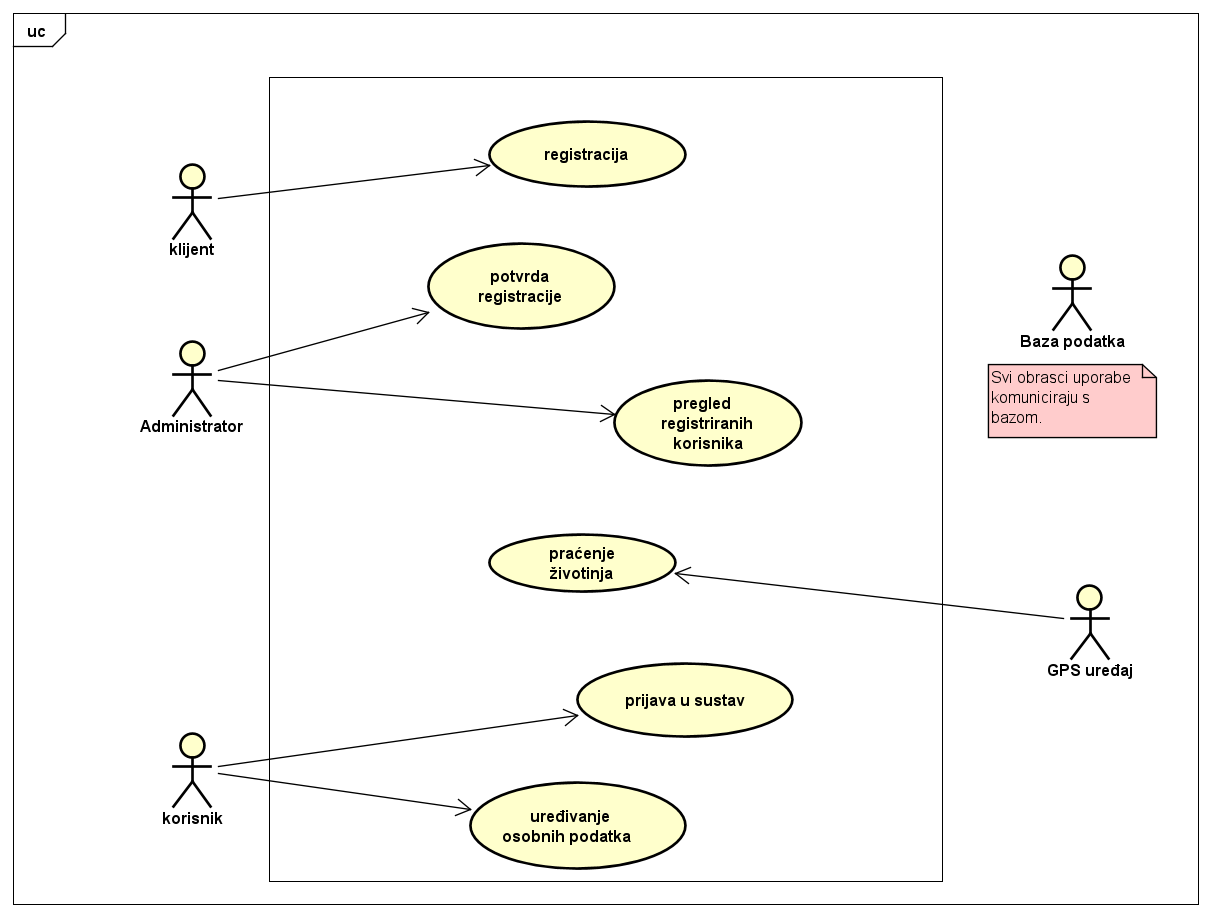
\includegraphics[scale=0.5]{slike/dijagram1.PNG} %veličina u odnosu na širinu linije
					\centering
					\caption{Dijagram obrasca uporabe, funkcionalnost administratora, klijenta, korisnika i GPS uređaja}
					\label{fig:dijagram1} %label mora biti drugaciji za svaku sliku
				\end{figure}
				
				\begin{figure}[H]
					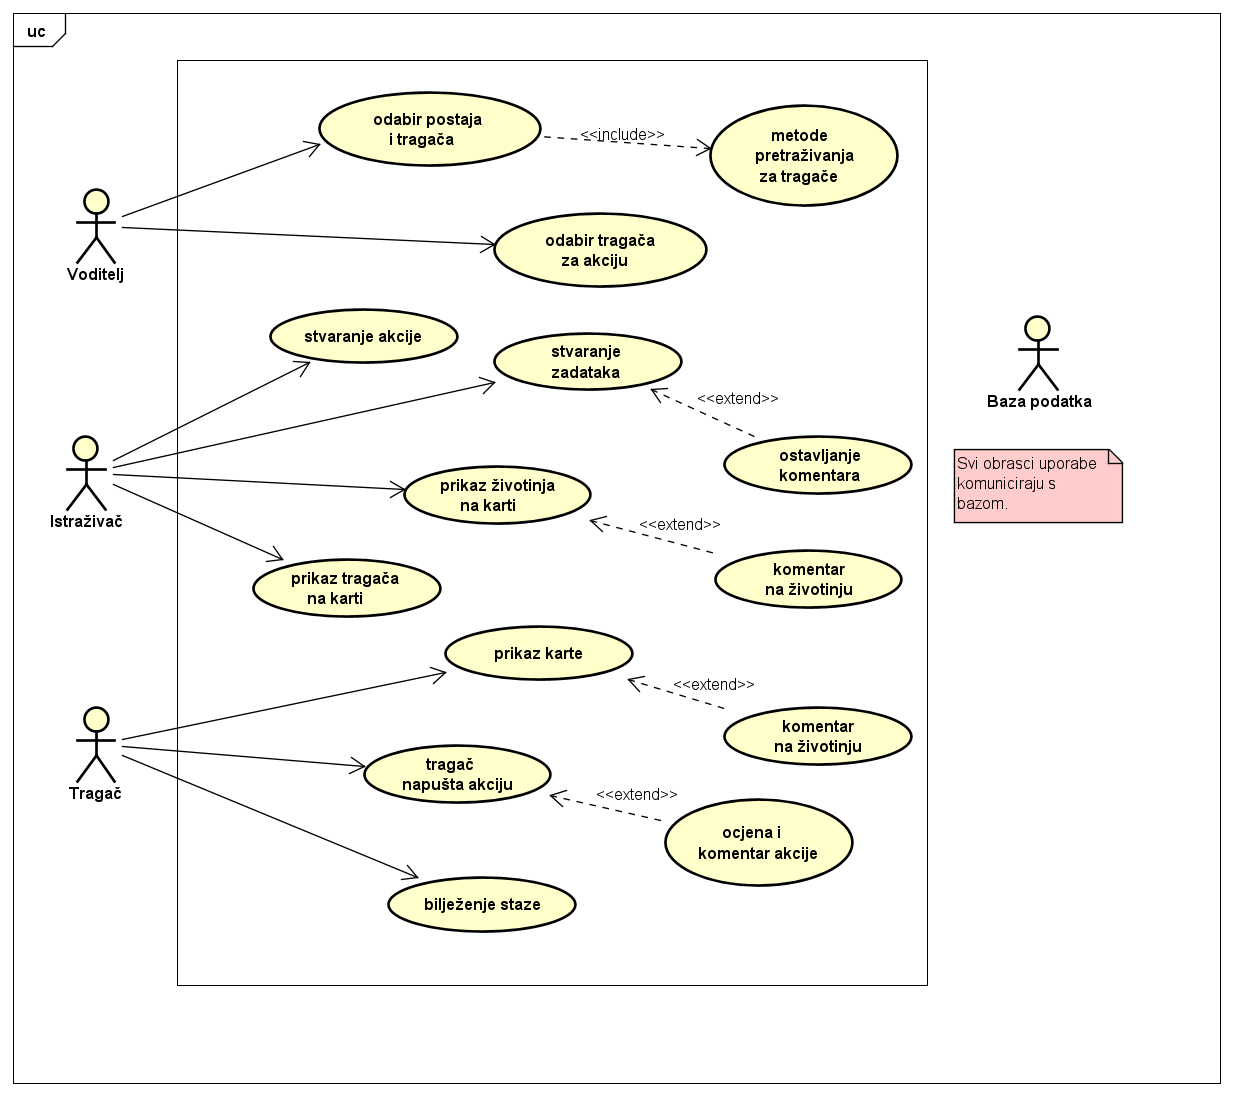
\includegraphics[scale=0.5]{slike/dijagram2.PNG} %veličina u odnosu na širinu linije
					\centering
					\caption{Dijagram obrasca uporabe, funkcionalnost voditelja, istraživača i tragača}
					\label{fig:dijagram2} %label mora biti drugaciji za svaku sliku
				\end{figure}
				
			\subsection{Sekvencijski dijagrami}
				
				\textbf{\textit{dio 1. revizije}}\\
				
				\textit{Nacrtati sekvencijske dijagrame koji modeliraju najvažnije dijelove sustava (max. 4 dijagrama). Ukoliko postoji nedoumica oko odabira, razjasniti s asistentom. Uz svaki dijagram napisati detaljni opis dijagrama.}\\
				
				\noindent \textbf{Obrazac uporabe UC6 - Voditelj odabire svoje postaje i tragače}\\
				
				\noindent Voditelj šalje zahtjev za prikaz stranice za odabir postaje i tragača. Poslužitelj prima zahtjev i iz baze podataka dohvaća dostupne tragače te prikazuje traženu stranicu voditelju. Voditelj odabire željenu postaju i tragače koji će biti vezani za tu postaju te potvrđuje svoj odabir. Poslužitelj prima potvrdu i sprema podatke o voditelju, postaji i tragačima u bazu podataka. Baza vraća potvrdu, a poslužitelj voditelju prikazuje stranicu s informacijama o njegovoj postaji.
				
				\begin{figure}[H]
					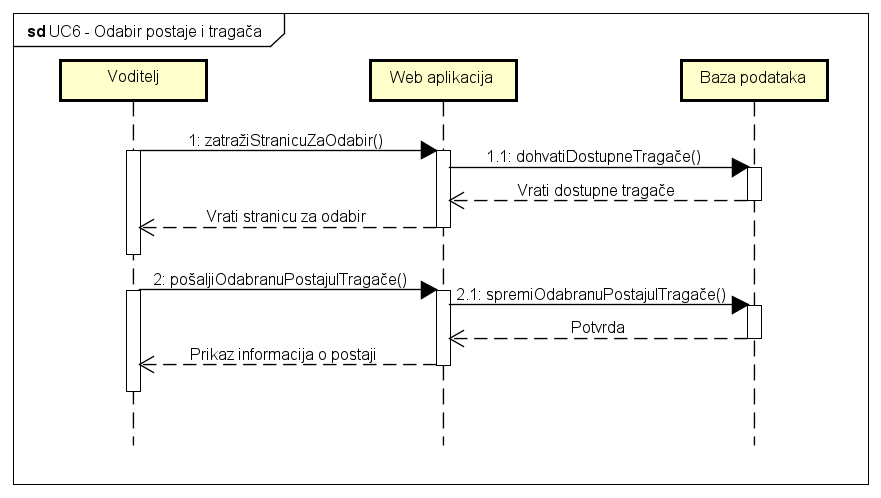
\includegraphics[scale=0.7]{slike/UC6_sekv.PNG} %veličina slike u odnosu na originalnu datoteku i pozicija slike
					\centering
					\caption{Sekvencijski dijagram - UC6}
					\label{fig:promjene}
				\end{figure}
				\eject
				
				\noindent \textbf{Obrazac uporabe UC7 - Voditelj definira metode pretraživanja igrača}\\
				
				\noindent Voditelj šalje zahtjev za prikaz stranice s popisom tragača i njihovih trenutnih metoda pretraživanja. Poslužitelj prima zahtjev te iz baze podataka dohvaća odabrane tragače i njihove metode pretraživanja i prikazuje voditelju stranicu za promjenu metoda pretraživanja. Ako tragač nema odabranu metodu, nedostupan je za akcije i voditelju je to naznačeno posebnom porukom te je potrebno odabrati neku metodu. Voditelj odabire metode pretraživanja svim željenim tragačima te šalje nove podatke poslužitelju. Postlužitelj te podatke šalje u bazu podataka koja vraća poruku potvrde, a poslužitelj voditelju prikazuje stranicu s informacijamao njegovoj postaji.
				
				\begin{figure}[H]
					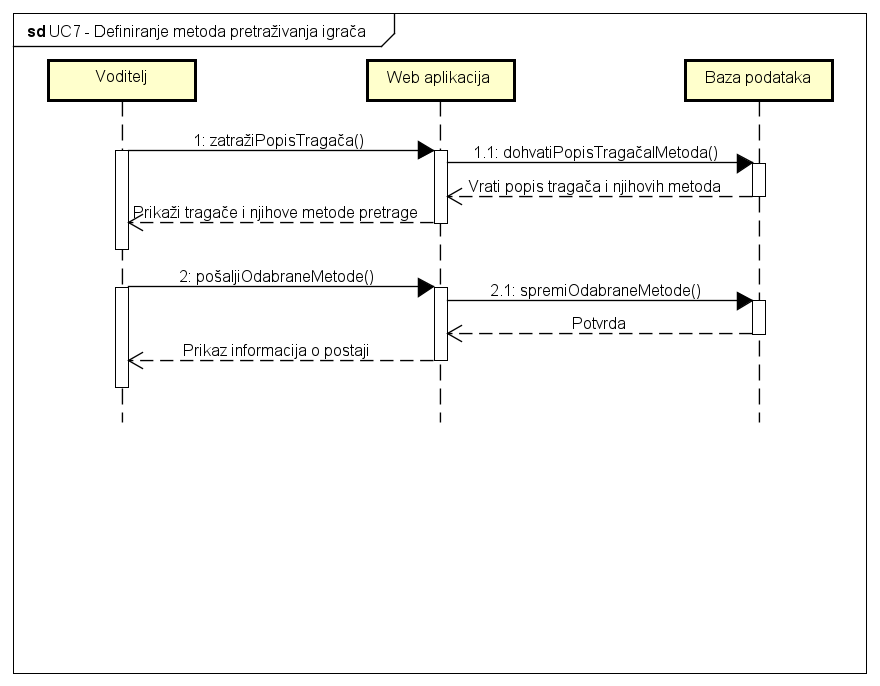
\includegraphics[scale=0.7]{slike/UC7_sekv.PNG} %veličina slike u odnosu na originalnu datoteku i pozicija slike
					\centering
					\caption{Sekvencijski dijagram - UC7}
					\label{fig:promjene}
				\end{figure}
				\eject
				
				\noindent \textbf{Obrazac uporabe UC11 - Stvaranje zadataka}\\
				
				\noindent Istraživač šalje zahtjev za prikazom stranice za dodjelu zadataka. Poslužitelj dohvaća dostupne tragače iz baze podataka te ih prikazuje istraživaču. Istraživač dodjeljuje zadatke za svakog tragača posebno(prolazak određenom rutom, dolazak do određene lokacije, postavljanje kamere ili uređaja za praćenje) upisom u formu pojedinačnog tragača. Nakon dodjele zadataka istraživač šalje zahtjev za spremanjem podataka. Poslužitelj prima zahtjev i šalje podatke o tragačima i zadatcima u bazu podataka. Poslužitelj odgovara porukom da je sve uspjelo.
				
				\begin{figure}[H]
					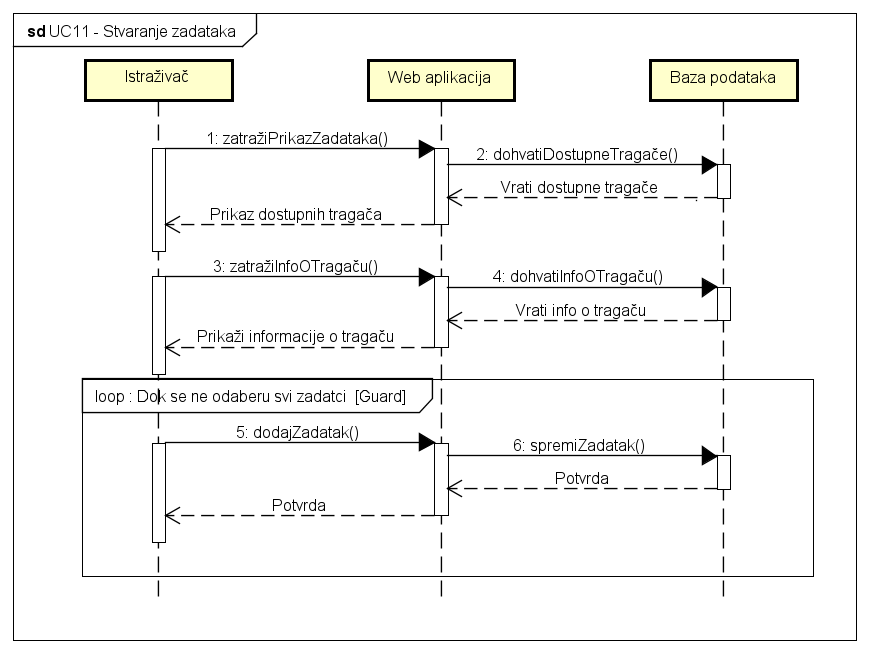
\includegraphics[scale=0.7]{slike/UC11_sekv.PNG} %veličina slike u odnosu na originalnu datoteku i pozicija slike
					\centering
					\caption{Sekvencijski dijagram - UC11}
					\label{fig:promjene}
				\end{figure}
				\eject
				
				\noindent \textbf{Obrazac uporabe UC15 - Prikaz karte za tragača}\\
				
				\noindent Tragač šalje zahtjev za prikazom stranice za odabir karte. Poslužitelj prima zahtjev, iz baze podataka dohvaća podatke o dostupnim akcijama te tragaču prikazuje stranicu na kojoj može odabrati kartu za određenu akciju te način prikaza informacija na karti (Popis zadataka, trenutne pozicije ostalih tragača, trenutne pozicije životinja). Ako tragač odabere popis zadataka, prikazuju mu se njegovi zadatci te ih može pregledati i označiti odrađenim. Ako tragač odabere prikaz karte i trenutnih pozicija, poslužitelj prima zahtjev, dohvaća podatke o pozicijama iz baze podataka i tragaču šalje stranicu na kojoj se prikazuje karta sa svim traženim pozicijama.
				
				\begin{figure}[H]
					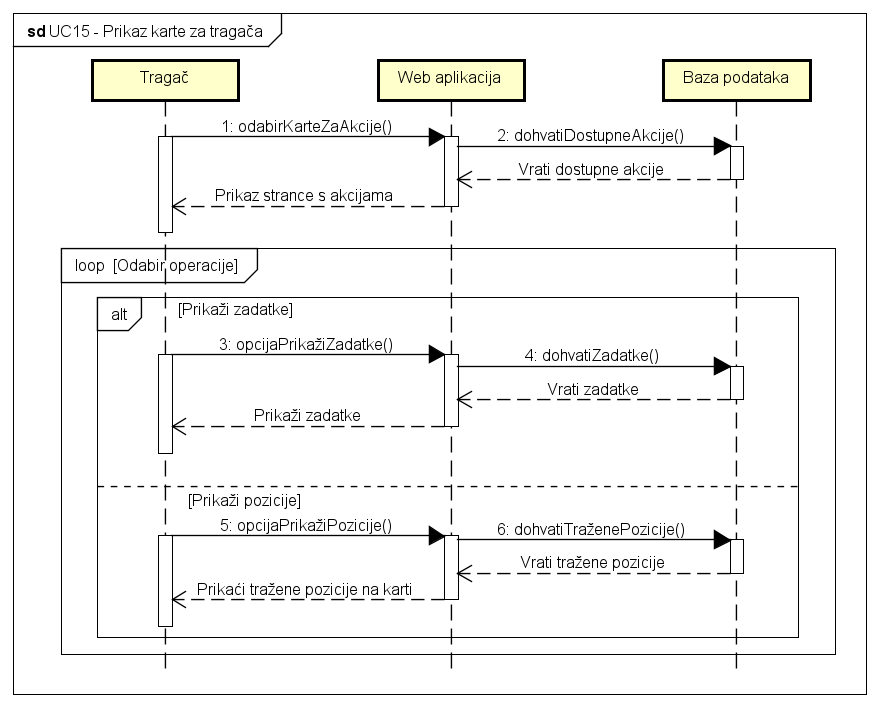
\includegraphics[scale=0.7]{slike/UC15_sekv.PNG} %veličina slike u odnosu na originalnu datoteku i pozicija slike
					\centering
					\caption{Sekvencijski dijagram - UC15}
					\label{fig:promjene}
				\end{figure}
	
		\section{Ostali zahtjevi}
		
			\textbf{\textit{dio 1. revizije}}\\
		 
			 \textit{Nefunkcionalni zahtjevi i zahtjevi domene primjene dopunjuju funkcionalne zahtjeve. Oni opisuju \textbf{kako se sustav treba ponašati} i koja \textbf{ograničenja} treba poštivati (performanse, korisničko iskustvo, pouzdanost, standardi kvalitete, sigurnost...). Primjeri takvih zahtjeva u Vašem projektu mogu biti: podržani jezici korisničkog sučelja, vrijeme odziva, najveći mogući podržani broj korisnika, podržane web/mobilne platforme, razina zaštite (protokoli komunikacije, kriptiranje...)... Svaki takav zahtjev potrebno je navesti u jednoj ili dvije rečenice.}
			 
			 \begin{packed_item}
			 	\item Vrijeme odziva poslužitelja mora biti maksimalno 10 sekundi
			 	\item Ne smiju postojati neautorizirane naredbe od strane registriranih korisnika
			 	\item Neregistrirani korisnici ne smiju imati pristup informacijama akcija i karata
			 	\item Neplanirano korištenje korisničkog sučelja ne smije narušiti sigurnost podataka
			 	\item Stranica treba biti responzivna
			 	\item Pregledna i lagana navigacija po aplikaciji
			 	\item Prikaz se mora jednostavno i intuitivno prilagoditi veličini zaslona
			 	\item Aplikacija ne smije preopteretiti radnu memoriju
			 \end{packed_item}
			 
			 
			 
	
	\chapter{Arhitektura i dizajn sustava}
		
		
	\noindent Arhitektura prati model klijent – server koja omogućava fleksibilnost u razvoju i održavanju budući da backend i frontend mogu evolouirati neovisno jedno o drugome. Komunikacija se vrši putem HTTP protokola.
	React je korišten za izgradnju frontend-a (klijentske strane), Spring Boot kao backend server, a PostgreSQL kao sustav za upravljanje bazom podataka. Pri izradi korisničkog sučelja komponente su građene tako da su reaktivne i ažuriraju se automatski kada se stanje aplikacije promijeni. Za upravljanje navigacijom unutar aplikacije korišten je React Router.
	Spring Boot je korišten za izradu backend dijela aplikacije koji obuhvaća:
	
	\begin{itemize}
		\item poslovnu logiku - servisi komuniciraju s repozitorijima i drugim servisima kako bi izvršili operacije nad podacima
		\item RESTful API-je - Rest Controlleri su definirani kako bi se obradili API zahtjevi, mapirani kao RESTful endpointovi
		\item pristup PostgreSQL bazi podataka – za komunikaciju se definiraju JPA repozitoriji koji omogućavaju pristup i upravljanje podacima.
	\end{itemize}
	
	
	Korisnik putem WEB preglednika šalje zahtjev WEB poslužitelju. WEB poslužitelj omogućava komunikaciju između klijenta i aplikacije putem HTTP protokola. Ukratko, WEB poslužitelj pokreće aplikaciju te joj prosljeđuje korisnikove zahtjeve. Frontend šalje HTTP zahtjeve prema SpringBootu putem fetcha, a backend obrađuje zahtjeve, pristupa bazi podataka, izvršava logiku i vraća rezultat frontendu u obliku JSON objekta.  Aplikacija u konačnici vraća odgovor u obliku HTML dokumenta.
	
		\begin{figure}[H]
		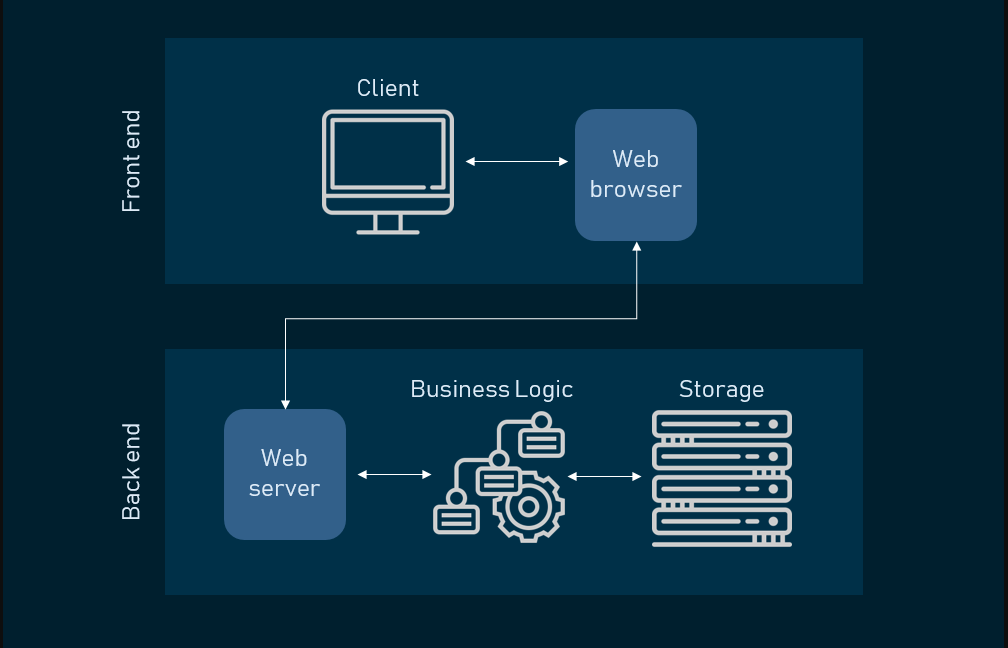
\includegraphics[scale=0.5]{slike/komunikacija.png} %veličina u odnosu na širinu linije
		\centering
		\caption{Komunikacija između frontenda i backenda}
		\label{fig:komunikacija} %label mora biti drugaciji za svaku sliku
		\end{figure}
	
				
		\section{Baza podataka}
			
				\noindent Za potrebe našeg sustava koristit ćemo relacijsku bazu podataka koja svojom strukturom olakšava modeliranje stvarnog svijeta. Temeljna jedinica baze je relacija, odnosno tablica koja je definirana svojim imenom i skupom atributa. Glavna svrha baze podataka je brza i jednostavna pohrana, izmjena i dohvaćanje podataka za daljnju obradu. Baza podataka ove aplikacije sastoji se od sljedećih entiteta:
				
				\begin{itemize}
					\item USER
					\item RESEARCHER
					\item MANAGER
					\item TRACKER
					\item ANIMAL
					\item STATION
					\item ACTION
					\item ACTION\_ANIMAL
					\item TASK
					\item MEDIUM
					\item QUALIFICATION
					\item TRACKER\_HISTORY
					\item ANIMAL\_HISTORY
					\item ROUTE
					\item ROUTE\_POINT
					\item ANIMAL\_COMMENT
					\item ACTION\_COMMENT
					\item ACTION\_HABITAT
					\item CONFIRMATION\_TOKEN
					\item HABITAT
					\item REQUEST
					\item REQUIREMENTS
					\item SPECIES
					\item TASK\_ANIMAL
					\item TASK\_COMMENT
					\item TRACKER\_ACTION\_MEDIUM
				\end{itemize}
				
		\subsection{Opis tablica}
				
				
				\noindent \textbf{USER} \hspace{1em} Ovaj entitet sadržava sve važne informacije vezane za korisnika aplikacije. Sadrži atribute ID korisnika, korisničko ime korisnika u aplikaciji, fotografiju korisnika, šifru računa korisnika, pravo ime i prezime korisnika, e-mail adresu, tip korisnika (istraživač, tragač ili voditelj stanice) i atribut koji označava je li korisnik registriran tipa BOOLEAN.  Ova klasa sadrži zajedničke atribute sva tri tipa korisnika aplikacije (voditelj, istraživač, tragač) te služi za lakše spremanje podataka koje svaki korisnik mora imati. Ovaj entitet je u vezi \textit{One-to-One} sa svakim tipom korisnika aplikacije. S klasom MAP\_COMMENT je u vezi \textit{One-to-Many} jer više korisnika (mora biti istraživač ili tragač) može ostaviti komentar na mapi.
				
				
				\begin{longtblr}[
					label=none,
					entry=none
					]{
						width = \textwidth,
						colspec={|X[6,l]|X[6, l]|X[20, l]|}, 
						rowhead = 1,
					} %definicija širine tablice, širine stupaca, poravnanje i broja redaka naslova tablice
					\hline \SetCell[c=3]{c}{\textbf{USER}}	 \\ \hline[3pt]
					\SetCell{LightGreen}id & INT	&  	jedinstveni identifikator (TRACKER.id ili MANAGER.id ili RESEARCHER.id)  	\\ \hline
					username & VARCHAR &   korisničko ime 	\\ \hline 
					photo & BYTEA & fotografija korisnika 	\\ \hline
					password & VARCHAR	& šifra korisničkog računa \\ \hline
					name & VARCHAR	& ime korisnika \\ \hline
					surname & VARCHAR & prezime korisnika \\ \hline
					email & VARCHAR & e-mail korisnika  \\ \hline 
					role & VARCHAR & tip korisnika  \\ \hline
					registered & BOOLEAN & oznaka koja definira je li korisnik registriran  \\ \hline
				\end{longtblr}
				
				
				\noindent \textbf{RESEARCHER} \hspace{1em} Ovaj entitet sadrži dodatni atribut odobrenja koji je potreban korisniku koji se odlučio za ulogu istraživača u aplikaciji. Povezan je s klasom USER vezom \textit{One-to-One} preko ID ključa. Dodatni atribut nam govori je li korisnik odobren kao istraživač od strane administratora jer je to preduvjet za obavljanje te uloge. U vezi je \textit{One-to-Many} s klasom ACTION (svaki istraživač može organizirati više radnih akcija). Također je s klasom ANIMAL\_COMMENT indirektno preko USER.id u vezi \textit{One-to-Many} jer više istraživača može ostaviti komentar na nekoj životinji.
				
				\begin{longtblr}[
					label=none,
					entry=none
					]{
						width = \textwidth,
						colspec={|X[6,l]|X[6, l]|X[20, l]|}, 
						rowhead = 1,
					} %definicija širine tablice, širine stupaca, poravnanje i broja redaka naslova tablice
					\hline \SetCell[c=3]{c}{\textbf{RESEARCHER}}	 \\ \hline[3pt]
					\SetCell{LightGreen}id & INT &	identifikator istraživača (USER.id)	\\ \hline
					approved & BOOLEAN & oznaka je li istraživač odobren od strane administratora\\ \hline
				\end{longtblr}				
				
				
				\noindent \textbf{MANAGER} \hspace{1em} Ovaj entitet sadrži dodatne atribute koji opisuju korisnika koji ima ulogu voditelja neke stanice. Moguće je da voditelj vodi samo jednu stanicu i također da jedna stanica ima samo jednog voditelja i zato je veza klase STATION i MANAGER \textit{One-to-One}. Dodatni atribut approved  označava je li korisniku odobren zahtjev za ulogu voditelja od strane administratora (isto kao kod istraživača) te atribut idStation označava jedinstveni identifikator stanice kojoj je korisnik voditelj.
				
				
				\begin{longtblr}[
					label=none,
					entry=none
					]{
						width = \textwidth,
						colspec={|X[6,l]|X[6, l]|X[20, l]|}, 
						rowhead = 1,
					} %definicija širine tablice, širine stupaca, poravnanje i broja redaka naslova tablice
					\hline \SetCell[c=3]{c}{\textbf{MANAGER}}	 \\ \hline[3pt]
					\SetCell{LightGreen}id & INT & jedinstveni identifikator (USER.id) \\ \hline
					approved & BOOLEAN & oznaka odobrenja \\ \hline
					\SetCell{LightBlue}idStation & INT & identifikator stanice (STATION.id) \\ \hline
				\end{longtblr}
				
				
				\noindent \textbf{TRACKER} \hspace{1em} Ovaj entitet označava korisnika koji obavlja ulogu tragača. Povezan je vezama \textit{One-to-One} s klasom USER i klasom TRACKER\_ACTION\_MEDIUM koja označava tragača koji trenutno obavlja zadatke neke akcije i vozilo kojim se koristi, te vezom \textit{Many-to-One} s klasom STATION i vezom \textit{One-to-Many} s klasom TASK jer jedan tragač može imati više zadataka. Tragač može obavljati zadatke koji su zadani od strane istraživača samo na jednoj stanici, dok stanica može imati više tragača na različitim zadatcima. S klasom ANIMAL\_COMMENT je indirektno preko USER.id u vezi \textit{One-to-Many} jer više tragača može ostaviti komentar na nekoj životinji. Sadrži atribute longitude i latitude koji služe za čuvanje zadnje poznate lokacije tragača.  Također je u vezi \textit{Many-to-Many} s klasom MEDIUM što se razrješava tablicom QUALIFICATION.
				
				\begin{longtblr}[
					label=none,
					entry=none
					]{
						width = \textwidth,
						colspec={|X[6,l]|X[6, l]|X[20, l]|}, 
						rowhead = 1,
					} %definicija širine tablice, širine stupaca, poravnanje i broja redaka naslova tablice
					\hline \SetCell[c=3]{c}{\textbf{TRACKER}}	 \\ \hline[3pt]
					\SetCell{LightGreen}id & INT & jedinstveni identifikator tragača (USER.id) \\ \hline
					longitude & DOUBLE & geografska dužina \\ \hline
					latitude & DOUBLE & geografska širina \\ \hline
					\SetCell{LightBlue} idStation & INT & jedinstveni identifikator stanice (STATION.id)\\ \hline
				\end{longtblr}
				
				\noindent \textbf{ANIMAL} \hspace{1em} Ovaj entitet predstavlja klasu životinja i sadrži sve atribute koji opisuju neku životinju. Sadrži atribute ID životinje, ID  vrste životinje, fotografiju životinje, ime jedinke, podatke o lokaciji i tekst koji opisuje životinju. U vezi je \textit{One-to-Many} s klasom  TASK jer na nekom zadatku se može pratiti jedna životinja dok više zadataka može pratiti istu životinju. S klasom ANIMAL\_COMMENT je u vezi \textit{One-to-Many} jer više komentara se može ostaviti za istu životinju. U \textit{One-to-Many} vezi je s klasom ANIMAL\_HISTORY koja sprema podatke o kretanju životinje. Također je u \textit{One-to-Many} vezi s klasom ACTION\_ANIMAL gdje se može vidjeti u kojim akcijama je životinja praćena. Još je u \textit{Many-to-Many} vezi s klasom ACTION što se dodatno razrješava u tablici ACTION\_ANIMAL.
				
				
				\begin{longtblr}[
					label=none,
					entry=none
					]{
						width = \textwidth,
						colspec={|X[6,l]|X[6, l]|X[20, l]|}, 
						rowhead = 1,
					} %definicija širine tablice, širine stupaca, poravnanje i broja redaka naslova tablice
					\hline \SetCell[c=3]{c}{\textbf{ANIMAL}}	 \\ \hline[3pt]
					\SetCell{LightGreen}id & INT & jedinstveni identifikator \\ \hline
					speciesId & INT & vrsta životinje \\ \hline
					photo & BYTEA & fotografija životinje \\ \hline
					description & TEXT & opis životinje \\ \hline
					longitude & DOUBLE & geografska dužina \\ \hline
					latitude & DOUBLE & geografska širina \\ \hline
					name & VARCHAR & ime jedinke \\ \hline
				\end{longtblr}
				
				
				
				\noindent \textbf{STATION} \hspace{1em} Ovaj entitet predstavlja klasu stanice koja sadrži atribute koje opisuju stanicu; ID stanice, ime stanice, podatke o lokaciji te kratki opis stanice. U vezi je \textit{One-to-One} s klasom MANAGER jer je za svaku stanicu zadužen je točno jedan voditelj te je u vezi \textit{One-to-Many} s klasom TRACKER jer više tragača može raditi za istu stanicu.
				
				\begin{longtblr}[
					label=none,
					entry=none
					]{
						width = \textwidth,
						colspec={|X[6,l]|X[6, l]|X[20, l]|}, 
						rowhead = 1,
					} %definicija širine tablice, širine stupaca, poravnanje i broja redaka naslova tablice
					\hline \SetCell[c=3]{c}{\textbf{STATION}}	 \\ \hline[3pt]
					\SetCell{LightGreen}id & INT & jedinstveni identifikator stanice \\ \hline
					longitude & DOUBLE & geografska dužina \\ \hline
					latitude & DOUBLE & geografska širina \\ \hline
					name & VARCHAR & ime stanice \\ \hline
					description & TEXT & opis stanice \\ \hline
				\end{longtblr}
				
				
				\noindent \textbf{ACTION} \hspace{1em} Ovaj entitet sadržava sve važne informacije vezane za akciju koju provodi određeni istraživač. Sadrži atribute ID, naslov, ID istraživača koji provodi akciju, ID voditelja postaje gdje se odvija akcija, vrijeme početka, vrijeme kraja te status  za trenutno stanje akcije (čeka da postane aktivna, na čekanju, riješena). Ovaj entitet u vezi je \textit{Many-to-One} s entitetom RESEARCHER preko ID-a istraživača te je u vezi \textit{One-to-Many} s entitetima TASK koji predstavlja zadatak, TRACKER\_ACTION\_MEDIUM koji predstavlja trenutno aktivne tragače u akcijama te njihov način prijevoza, ANIMAL\_COMMENT koji predstavlja komentar tragača vezan za određenu životinju u nekoj akciji te ACTION\_ANIMAL gdje se može vidjeti koje životinje se prate u akciji. Još je u \textit{Many-to-Many} vezi s entitetom HABITAT te ANIMAL što se dodatno razrješava u tablici ACTION\_ANIMAL.
				
				\begin{longtblr}[
					label=none,
					entry=none
					]{
						width = \textwidth,
						colspec={|X[6,l]|X[6, l]|X[20, l]|}, 
						rowhead = 1,
					} %definicija širine tablice, širine stupaca, poravnanje i broja redaka naslova tablice
					\hline \SetCell[c=3]{c}{\textbf{ACTION}}	 \\ \hline[3pt]
					\SetCell{LightGreen}id & INT & jedinstveni identifikator \\ \hline
					title & VARCHAR & naslov akcije \\ \hline
					\SetCell{LightBlue}idResearcher & INT & ID istraživača (RESEARCHER.id) \\ \hline
					\SetCell{LightBlue}idManager & INT & ID voditelja postaje (MANAGER.id) \\ \hline
					startOfAction & TIMESTAMP & vrijeme početka \\ \hline
					endOfAction & TIMESTAMP & vrijeme kraja \\ \hline
					status & INT & kodni broj za trenutno stanje akcije \\ \hline
				\end{longtblr}
				
				
				\noindent \textbf{ACTION\_ANIMAL} \hspace{1em} Ovaj entitet sadržava sve važne informacije vezane za praćene životinje u nekoj akciji te razrješava \textit{Many-to-Many} vezu između entiteta ANIMAL i ACTION. Sadrži atribute ID životinje te ID akcije u kojoj je ta životinja praćena. Ovaj entitet u vezi je \textit{Many-to-One} s entitetima ANIMAL preko ID-a životinje i ACTION preko ID-a akcije.
				
					\begin{longtblr}[
					label=none,
					entry=none
					]{
						width = \textwidth,
						colspec={|X[6,l]|X[6, l]|X[20, l]|}, 
						rowhead = 1,
					} %definicija širine tablice, širine stupaca, poravnanje i broja redaka naslova tablice
					\hline \SetCell[c=3]{c}{\textbf{ACTION\_ANIMAL}}	 \\ \hline[3pt]
					\SetCell{LightGreen}idAnimal & INT & ID životinje (ANIMAL.id), ujedno i prvi dio kompozitnog primarnog ključa \\ \hline
					\SetCell{LightGreen}idAction & INT & ID akcije (ACTION.id), ujedno i drugi dio kompozitnog primarnog ključa \\ \hline
				\end{longtblr}
				
				
				\noindent \textbf{TASK} \hspace{1em} Ovaj entitet sadržava sve važne informacije vezane za zadatak koji je dio neke akcije te ga odrađuje određeni tragač. Sadrži atribute ID, naslov, opis, ID tragača koji odrađuje zadatak, ID akcije kojoj pripada, trenutnu geografsku širinu i dužinu, geografsku lokaciju početka i kraja zadatka, ID rute za slučaj da je potreban prolazak nekom rutom, vrijeme početka, vrijeme početka i kraja te status koji za trenutno stanje zadatka (čeka da postane aktivan, riješen, prekinut). Ovaj entitet u vezi je \textit{Many-to-One} s entitetima RESEARCHER preko ID-a istraživača, ACTION preko ID-a akcije, ANIMAL preko ID-a životinje, ROUTE preko ID-a rute.
				
				\begin{longtblr}[
					label=none,
					entry=none
					]{
						width = \textwidth,
						colspec={|X[6,l]|X[6, l]|X[20, l]|}, 
						rowhead = 1,
					} %definicija širine tablice, širine stupaca, poravnanje i broja redaka naslova tablice
					\hline \SetCell[c=3]{c}{\textbf{TASK}}	 \\ \hline[3pt]
					\SetCell{LightGreen}id & INT & jedinstveni identifikator \\ \hline
					title & VARCHAR & naslov zadatka \\ \hline
					\SetCell{LightBlue}idTracker & INT & ID tragača (TRACKER.id) \\ \hline
					\SetCell{LightBlue}idAction & INT & ID akcije (ACTION.id) \\ \hline
					latitude & DOUBLE & geografska širina \\ \hline
					longitude & DOUBLE & geografska dužina \\ \hline
					latStart & DOUBLE & geografska širina početka zadatka \\ \hline
					lonStart & DOUBLE & geografska dužina početka zadatka \\ \hline
					latFinish & DOUBLE & geografska širina kraja zadatka \\ \hline
					lonFinish & DOUBLE & geografska dužina kraja zadatka \\ \hline
					\SetCell{LightBlue}idRoute & INT & ID rute (ROUTE.id) \\ \hline
					content & TEXT & opis (sadržaj) zadatka \\ \hline
					start & TIMESTAMP & vrijeme početka \\ \hline
					end & TIMESTAMP & vrijeme kraja \\ \hline
					status & TEXT & kodni broj za trenutno stanje zadatka \\ \hline
				\end{longtblr}
				
				
				
				\noindent \textbf{MEDIUM} \hspace{1em} Ovaj entitet sadržava sve važne informacije vezane za sredstva prijevoza koje tragači mogu koristiti u akcijama. Sadrži atribute tip (npr. automobil, zrakoplov…), zračna linija što je oznaka računa li se ruta do neke lokacije za taj tip prijevoza kao pravocrtna (zračna linija), radijus pretraživanja moguć s tim sredstvom, vrijednost na skali koliko dobro se uočavaju detalji s tim tipom sredstva te vrijednost na skali kolika je brzina putovanja tim tipom sredstva. Ovaj entitet u vezi je \textit{Many-to-Many} s entitetom TRACKER što se dodatno razrješava u tablici QUALIFICATION te je u vezi \textit{One-to-Many} s entitetima TRACKER\_ACTION\_MEDIUM te QUALIFICATION.
				
				\begin{longtblr}[
					label=none,
					entry=none
					]{
						width = \textwidth,
						colspec={|X[6,l]|X[6, l]|X[20, l]|}, 
						rowhead = 1,
					} %definicija širine tablice, širine stupaca, poravnanje i broja redaka naslova tablice
					\hline \SetCell[c=3]{c}{\textbf{MEDIUM}}	 \\ \hline[3pt]
					\SetCell{LightGreen}type & VARCHAR & tip sredstva prijevoza, ujedno i primarni ključ \\ \hline
					airline & BOOLEAN & oznaka računa li se pravocrtna ruta \\ \hline
					radius & DOUBLE & mogući radijus pretraživanja \\ \hline
					detail & DOUBLE & vrijednost na skali koliko dobro se uočavaju detalji \\ \hline
					speed & DOUBLE & vrijednost na skali kolika je brzina putovanja \\ \hline
				\end{longtblr}
				
				\noindent \textbf{QUALIFICATION} \hspace{1em} Ovaj entitet sadržava sve važne informacije vezane za kvalifikacije tragača za tip sredstva prijevoza te razrješava \textit{Many-to-Many} vezu između entiteta TRACKER i MEDIUM. Sadrži atribute ID tragača te tip sredstva prijevoza za koje je taj tragač kvalificiran. Ovaj entitet u vezi je \textit{Many-to-One} s entitetima TRACKER preko ID-a tragača i MEDIUM preko tipa sredstva prijevoza.
				
				\begin{longtblr}[
					label=none,
					entry=none
					]{
						width = \textwidth,
						colspec={|X[6,l]|X[6, l]|X[20, l]|}, 
						rowhead = 1,
					} %definicija širine tablice, širine stupaca, poravnanje i broja redaka naslova tablice
					\hline \SetCell[c=3]{c}{\textbf{QUALIFICATION}}	 \\ \hline[3pt]
					\SetCell{LightGreen}idTracker & INT & ID tragača (TRACKER.id), ujedno i prvi dio kompozitnog primarnog ključa \\ \hline
					\SetCell{LightGreen}typeMedium & VARCHAR & tip (ujedno i ID) sredstva prijevoza (MEDIUM.type), ujedno i drugi dio kompozitnog primarnog ključa \\ \hline
				\end{longtblr}
				
				\noindent \textbf{TRACKER\_ACTION\_MEDIUM} \hspace{1em} Ovaj entitet sadržava sve važne informacije vezane za odnos trenutno aktivnih akcija i tragača koji rade na njima. Sadrži atribute ID, ID tragača, ID akcije te sredstvo prijevoza. Ovaj entitet u vezi je \textit{One-to-One} s entitetom TRACKER preko ID-a tragača te je u vezi \textit{Many-to-One} s entitetima ACTION preko ID-a akcije, MEDIUM preko tipa sredstva prijevoza.
				
				\begin{longtblr}[
					label=none,
					entry=none
					]{
						width = \textwidth,
						colspec={|X[6,l]|X[6, l]|X[20, l]|}, 
						rowhead = 1,
					} %definicija širine tablice, širine stupaca, poravnanje i broja redaka naslova tablice
					\hline \SetCell[c=3]{c}{\textbf{TRACKER\_ACTION\_MEDIUM}}	 \\ \hline[3pt]
					\SetCell{LightGreen}id & INT & jedinstveni identifikator \\ \hline
					\SetCell{LightBlue}idTracker & INT & ID tragača (TRACKER.id), ujedno i primarni ključ \\ \hline
					\SetCell{LightBlue}idAction & INT & ID akcije (ACTION.id) \\ \hline
					\SetCell{LightBlue}typeMedium & VARCHAR & tip (ujedno i ID) sredstva prijevoza (MEDIUM.type) \\ \hline
				\end{longtblr}
				
			
				
				
				\noindent \textbf{TRACKER\_HISTORY} \hspace{1em} Ova tablica bilježi podatke na mapi, odnosno točke na mapi kojima je tragač prolazio tijekom obavljanja zadataka. U vezi je \textit{Many-to-One} s tablicom TRACKER što znači da za jednog tragača može biti više zabilježenih točaka na mapi. Atributi su ID, ID tragača, vrijeme bilježenja lokacije te zemljopisna dužina i širina.
				
				\begin{longtblr}[
					label=none,
					entry=none
					]{
						width = \textwidth,
						colspec={|X[6,l]|X[6, l]|X[20, l]|}, 
						rowhead = 1,
					} %definicija širine tablice, širine stupaca, poravnanje i broja redaka naslova tablice
					\hline \SetCell[c=3]{c}{\textbf{TRACKER\_HISTORY}}	 \\ \hline[3pt]
					\SetCell{LightGreen}id & INT & jedinstveni identifikator \\ \hline
					\SetCell{LightBlue}idTracker & INT & identifikator tragača (TRACKER.id) \\ \hline
					time & TIMESTAMP & vrijeme bilježenja lokacije \\ \hline
					latitude & DOUBLE & zemljopisna širina \\ \hline
					longitude & DOUBLE & zemljopisna dužina \\ \hline
				\end{longtblr}
				
				
				\noindent \textbf{ANIMAL\_HISTORY} \hspace{1em} Ova tablica zapisane lokacije na kojima je određena životinja prolazila u nekom trenutku. Sadrži atribute ID životinje, vrijeme bilježenja lokacije, zemljopisnu širinu i dužinu.Atributi su ID, ID životinje, vrijeme bilježenja lokacije te zemljopisna dužina i širina. Entitet je u vezi \textit{Many-to-One} s tablicom ANIMAL zato jer se za jednu životinju može zabilježiti više točaka na karti.
				
				\begin{longtblr}[
					label=none,
					entry=none
					]{
						width = \textwidth,
						colspec={|X[6,l]|X[6, l]|X[20, l]|}, 
						rowhead = 1,
					} %definicija širine tablice, širine stupaca, poravnanje i broja redaka naslova tablice
					\hline \SetCell[c=3]{c}{\textbf{ANIMAL\_HISTORY}}	 \\ \hline[3pt]
					\SetCell{LightGreen}id & INT & jedinstveni identifikator \\ \hline
					\SetCell{LightBlue}idAnimal & INT & identifikator životinje (ANIMAL.id) \\ \hline
					time & TIMESTAMP & vrijeme bilježenja lokacije \\ \hline
					latitude & DOUBLE & zemljopisna širina \\ \hline
					longitude & DOUBLE & zemljopisna dužina \\ \hline
				\end{longtblr}
				
				
				
				\noindent \textbf{ANIMAL\_COMMENT} \hspace{1em} Ovaj entitet sadržava sve važne informacije vezane za komentar nekog tragača o nekoj životinji u nekoj akciji. Sadrži atribute ID, naslov, ID životinje na koju se komentar odnosi, ID tragača koji je napisao komentar, ID akcije u kojoj je komentar napisan, vrijeme izrade te sadržaj komentara. Ovaj entitet u vezi je \textit{Many-to-One} s entitetima ANIMAL preko ID-a životinje, USER preko ID-a korisnika (može biti TRACKER ili RESEARCHER) te ACTION preko ID-a akcije.
				
				\begin{longtblr}[
					label=none,
					entry=none
					]{
						width = \textwidth,
						colspec={|X[6,l]|X[6, l]|X[20, l]|}, 
						rowhead = 1,
					} %definicija širine tablice, širine stupaca, poravnanje i broja redaka naslova tablice
					\hline \SetCell[c=3]{c}{\textbf{ANIMAL\_COMMENT}}	 \\ \hline[3pt]
					\SetCell{LightGreen}id & INT & jedinstveni identifikator \\ \hline
					title & VARCHAR & naslov komentara \\ \hline
					\SetCell{LightBlue}idAnimal & INT & ID životinje (ANIMAL.id) \\ \hline
					\SetCell{LightBlue}idUser & INT & ID korisnika (USER.id, indirektno povezano s TRACKER.id ili RESEARCHER.id) \\ \hline
					\SetCell{LightBlue}idAction & INT & ID akcije (ACTION.id) \\ \hline
					time & TIMESTAMP & vrijeme izrade \\ \hline
					content & TEXT & sadržaj komentara \\ \hline
				\end{longtblr}
				
				\noindent \textbf{ACTION\_COMMENT} \hspace{1em} Ovaj entitet sadržava sve važne informacije vezane za komentar nekog istraživača ili tragača o nekoj nekoj akciji. Sadrži atribute ID, naslov, ID akcije na koju se komentar odnosi, ID korisnika koji je napisao komentar, vrijeme izrade te sadržaj komentara. Ovaj entitet u vezi je \textit{Many-to-One} s entitetima ACTION preko ID-a akcije te USER preko ID-a korisnika (može biti TRACKER ili RESEARCHER).
				
				\begin{longtblr}[
					label=none,
					entry=none
					]{
						width = \textwidth,
						colspec={|X[6,l]|X[6, l]|X[20, l]|}, 
						rowhead = 1,
					} %definicija širine tablice, širine stupaca, poravnanje i broja redaka naslova tablice
					\hline \SetCell[c=3]{c}{\textbf{ACTION\_COMMENT}}	 \\ \hline[3pt]
					\SetCell{LightGreen}id & INT & jedinstveni identifikator \\ \hline
					title & VARCHAR & naslov komentara \\ \hline
					\SetCell{LightBlue}idUser & INT & ID korisnika (USER.id, indirektno povezano s TRACKER.id ili RESEARCHER.id) \\ \hline
					\SetCell{LightBlue}idAction & INT & ID akcije (ACTION.id) \\ \hline
					time & TIMESTAMP & vrijeme izrade \\ \hline
					content & TEXT & sadržaj komentara \\ \hline
				\end{longtblr}
				
				\noindent \textbf{TASK\_COMMENT} \hspace{1em} Ovaj entitet sadržava sve važne informacije vezane za komentar nekog tragača ili istraživača o nekom zadatku u nekoj akciji. Sadrži atribute ID, naslov, ID zadatka na koji se komentar odnosi, ID korisnika koji je napisao komentar, vrijeme izrade te sadržaj komentara. Ovaj entitet u vezi je \textit{Many-to-One} s entitetima TASK preko ID-a zadatka i preko njega inidirektno i s ACTION te USER preko ID-a korisnika (može biti TRACKER ili RESEARCHER).
				
				\begin{longtblr}[
					label=none,
					entry=none
					]{
						width = \textwidth,
						colspec={|X[6,l]|X[6, l]|X[20, l]|}, 
						rowhead = 1,
					} %definicija širine tablice, širine stupaca, poravnanje i broja redaka naslova tablice
					\hline \SetCell[c=3]{c}{\textbf{TASK\_COMMENT}}	 \\ \hline[3pt]
					\SetCell{LightGreen}id & INT & jedinstveni identifikator \\ \hline
					title & VARCHAR & naslov komentara \\ \hline
					\SetCell{LightBlue}idTask & INT & ID zadatka (TASK.id) \\ \hline
					\SetCell{LightBlue}idUser & INT & ID korisnika (USER.id, indirektno povezano s TRACKER.id ili RESEARCHER.id) \\ \hline
					time & TIMESTAMP & vrijeme izrade \\ \hline
					content & TEXT & sadržaj komentara \\ \hline
				\end{longtblr}
				
				\noindent \textbf{ACTION\_HABITAT} \hspace{1em} Ovaj entitet sadržava sve važne informacije vezane za praćene životinje u nekom staništu te razrješava \textit{Many-to-Many} vezu između entiteta ANIMAL i HABITAT. Sadrži atribute ID staništa te ID akcije u kojoj je ta životinja praćena. Ovaj entitet u vezi je \textit{Many-to-One} s entitetima HABITAT preko ID-a staništa i ACTION preko ID-a akcije.
				
				\begin{longtblr}[
					label=none,
					entry=none
					]{
						width = \textwidth,
						colspec={|X[6,l]|X[6, l]|X[20, l]|}, 
						rowhead = 1,
					} %definicija širine tablice, širine stupaca, poravnanje i broja redaka naslova tablice
					\hline \SetCell[c=3]{c}{\textbf{ACTION\_HABITAT}}	 \\ \hline[3pt]
					\SetCell{LightGreen}idHabitat & INT & ID staništa (HABITAT.id), ujedno i prvi dio kompozitnog primarnog ključa \\ \hline
					\SetCell{LightGreen}idAction & INT & ID akcije (ACTION.id), ujedno i drugi dio kompozitnog primarnog ključa \\ \hline
				\end{longtblr}
				
				\noindent \textbf{CONFIRMATION\_TOKEN} \hspace{1em} Ovaj entitet sadržava sve važne informacije vezane za kreiranje tokena radi sigurnije prijave korisnika pomoću potvrde email adrese. Sadrži atribute ID, tekst koji je sifra tokena, vremena kreiranja, potvrdivanja i isteka tokena te strani ključ idUser. Ovaj entitet u vezi je \textit{Many-to-One} s entitetom USER preko ID-a korisnika.
				
				\begin{longtblr}[
					label=none,
					entry=none
					]{
						width = \textwidth,
						colspec={|X[6,l]|X[6, l]|X[20, l]|}, 
						rowhead = 1,
					} %definicija širine tablice, širine stupaca, poravnanje i broja redaka naslova tablice
					\hline \SetCell[c=3]{c}{\textbf{CONFIRMATION\_TOKEN}}	 \\ \hline[3pt]
					\SetCell{LightGreen}id & INT & tip sredstva prijevoza, ujedno i primarni ključ \\ \hline
					\SetCell{LightBlue}idUser & INT & ID korisnika (USER.id) \\ \hline
					createdAt & TIMESTAMP & vrijeme izrade \\ \hline
					confirmedAt & TIMESTAMP & vrijeme potvrde \\ \hline
					expiresAt & TIMESTAMP & vrijeme isteka \\ \hline
					token & TEXT & šifra tokena \\ \hline
					
				\end{longtblr}
				
				\noindent \textbf{SPECIES} \hspace{1em} Ovaj entitet predstavlja klasu vrsta životinja i sadrži sve atribute koji opisuju neku vrstu. Sadrži atribute ID, fotografiju vrste, ime vrste i tekst koji opisuje životinju. U vezi je \textit{One-to-Many} s klasom  ANIMAL jer jedna vrsta može imati više jediniki životinja, a jedna jedinka može biti samo jedne  vrste.
				
				
				\begin{longtblr}[
					label=none,
					entry=none
					]{
						width = \textwidth,
						colspec={|X[6,l]|X[6, l]|X[20, l]|}, 
						rowhead = 1,
					} %definicija širine tablice, širine stupaca, poravnanje i broja redaka naslova tablice
					\hline \SetCell[c=3]{c}{\textbf{SPECIES}}	 \\ \hline[3pt]
					\SetCell{LightGreen}id & INT & jedinstveni identifikator \\ \hline
					photo & BYTEA & fotografija vrste \\ \hline
					description & TEXT & opis vrste \\ \hline
					name & VARCHAR & ime vrste \\ \hline
				\end{longtblr}
				
				
				\noindent \textbf{HABITAT} \hspace{1em} Ovaj entitet predstavlja klasu različitih staništa i sadrži sve atribute koji opisuju neko stanište. Sadrži atribute ID, fotografiju staništa, ime staništa, tekst koji opisuje stanište, radijus koji obuhvaća stanište te geografsku lokaciju staništa. U vezi je \textit{One-to-Many} s klasom ANIMAL jedno stanište može biti stanište više životinja, a jedna životinja ima isključivo to stanište te je u vezi  \textit{One-to-Many} s klasom ACTION jer jedna akcija može imati više staništa, a stanište može biti dio više akcija. 
				
				
				\begin{longtblr}[
					label=none,
					entry=none
					]{
						width = \textwidth,
						colspec={|X[6,l]|X[6, l]|X[20, l]|}, 
						rowhead = 1,
					} %definicija širine tablice, širine stupaca, poravnanje i broja redaka naslova tablice
					\hline \SetCell[c=3]{c}{\textbf{HABITAT}}	 \\ \hline[3pt]
					\SetCell{LightGreen}id & INT & jedinstveni identifikator \\ \hline
					photo & BYTEA & fotografija staništa \\ \hline
					description & TEXT & opis staništa \\ \hline
					name & VARCHAR & ime staništa \\ \hline
					radius & DOUBLE & radijus staništa \\ \hline
					latitude & DOUBLE & geografska širina \\ \hline
					longitude & DOUBLE & geografska dužina \\ \hline
				\end{longtblr}
				
				\noindent \textbf{REQUEST} \hspace{1em} Ovaj entitet sadržava sve važne informacije vezane za zahtjev unutar određene akcije. Sadrži atribute ID, ID korisnika koji je kreirao zahtjev, ID akcije, tip zahtjeva, status zahtjeva te vrijeme izrade. Ovaj entitet u vezi je \textit{One-to-One} s entitetom USER preko ID-a korisnika te je u vezi \textit{Many-to-one} s entitetom ACTION koji predstavlja akciju.
				
				\begin{longtblr}[
					label=none,
					entry=none
					]{
						width = \textwidth,
						colspec={|X[6,l]|X[6, l]|X[20, l]|}, 
						rowhead = 1,
					} %definicija širine tablice, širine stupaca, poravnanje i broja redaka naslova tablice
					\hline \SetCell[c=3]{c}{\textbf{REQUEST}}	 \\ \hline[3pt]
					\SetCell{LightGreen}id & INT & jedinstveni identifikator \\ \hline
					\SetCell{LightBlue}idResearcher & INT & ID korisnika (USER.id) \\ \hline
					\SetCell{LightBlue}idAction & INT & ID akcije (ACTION.id) \\ \hline
					creationTime & TIMESTAMP & vrijeme izrade \\ \hline
					status & VARCHAR &  trenutno stanje akcije \\ \hline
					type & VARCHAR & tip zahtjeva \\ \hline
					
				\end{longtblr}
				
				\noindent \textbf{REQUIREMENTS} \hspace{1em} Ovaj entitet sadržava sve važne informacije vezane za specifične uvjete koje voditelj traži za pojedinu akciju. Sadrži atribute ID akcije, vrstu vozila tragača i količinu tih pojedinih tragača potrebnih za akciju. Ovaj entitet u vezi je \textit{One-to-One} s entitetom ACTION preko ID-a akcije.
				
				\begin{longtblr}[
					label=none,
					entry=none
					]{
						width = \textwidth,
						colspec={|X[6,l]|X[6, l]|X[20, l]|}, 
						rowhead = 1,
					} %definicija širine tablice, širine stupaca, poravnanje i broja redaka naslova tablice
					\hline \SetCell[c=3]{c}{\textbf{REQUIREMENTS}}	 \\ \hline[3pt]
					\SetCell{LightBlue}idAction & INT & ID akcije (ACTION.id) \\ \hline
					amount & INT & broj tragača s pojedinim vozilom \\ \hline
					type & VARCHAR & tragaci s traženim tipom vozila \\ \hline
				\end{longtblr}
		
				
				
												
				
			\eject
			
				
			\iffalse
						
			\subsection{Dijagram baze podataka}
								
				
				\newgeometry{margin=0pt}			
				\begin{figure}
					\vspace{\baselineskip}
					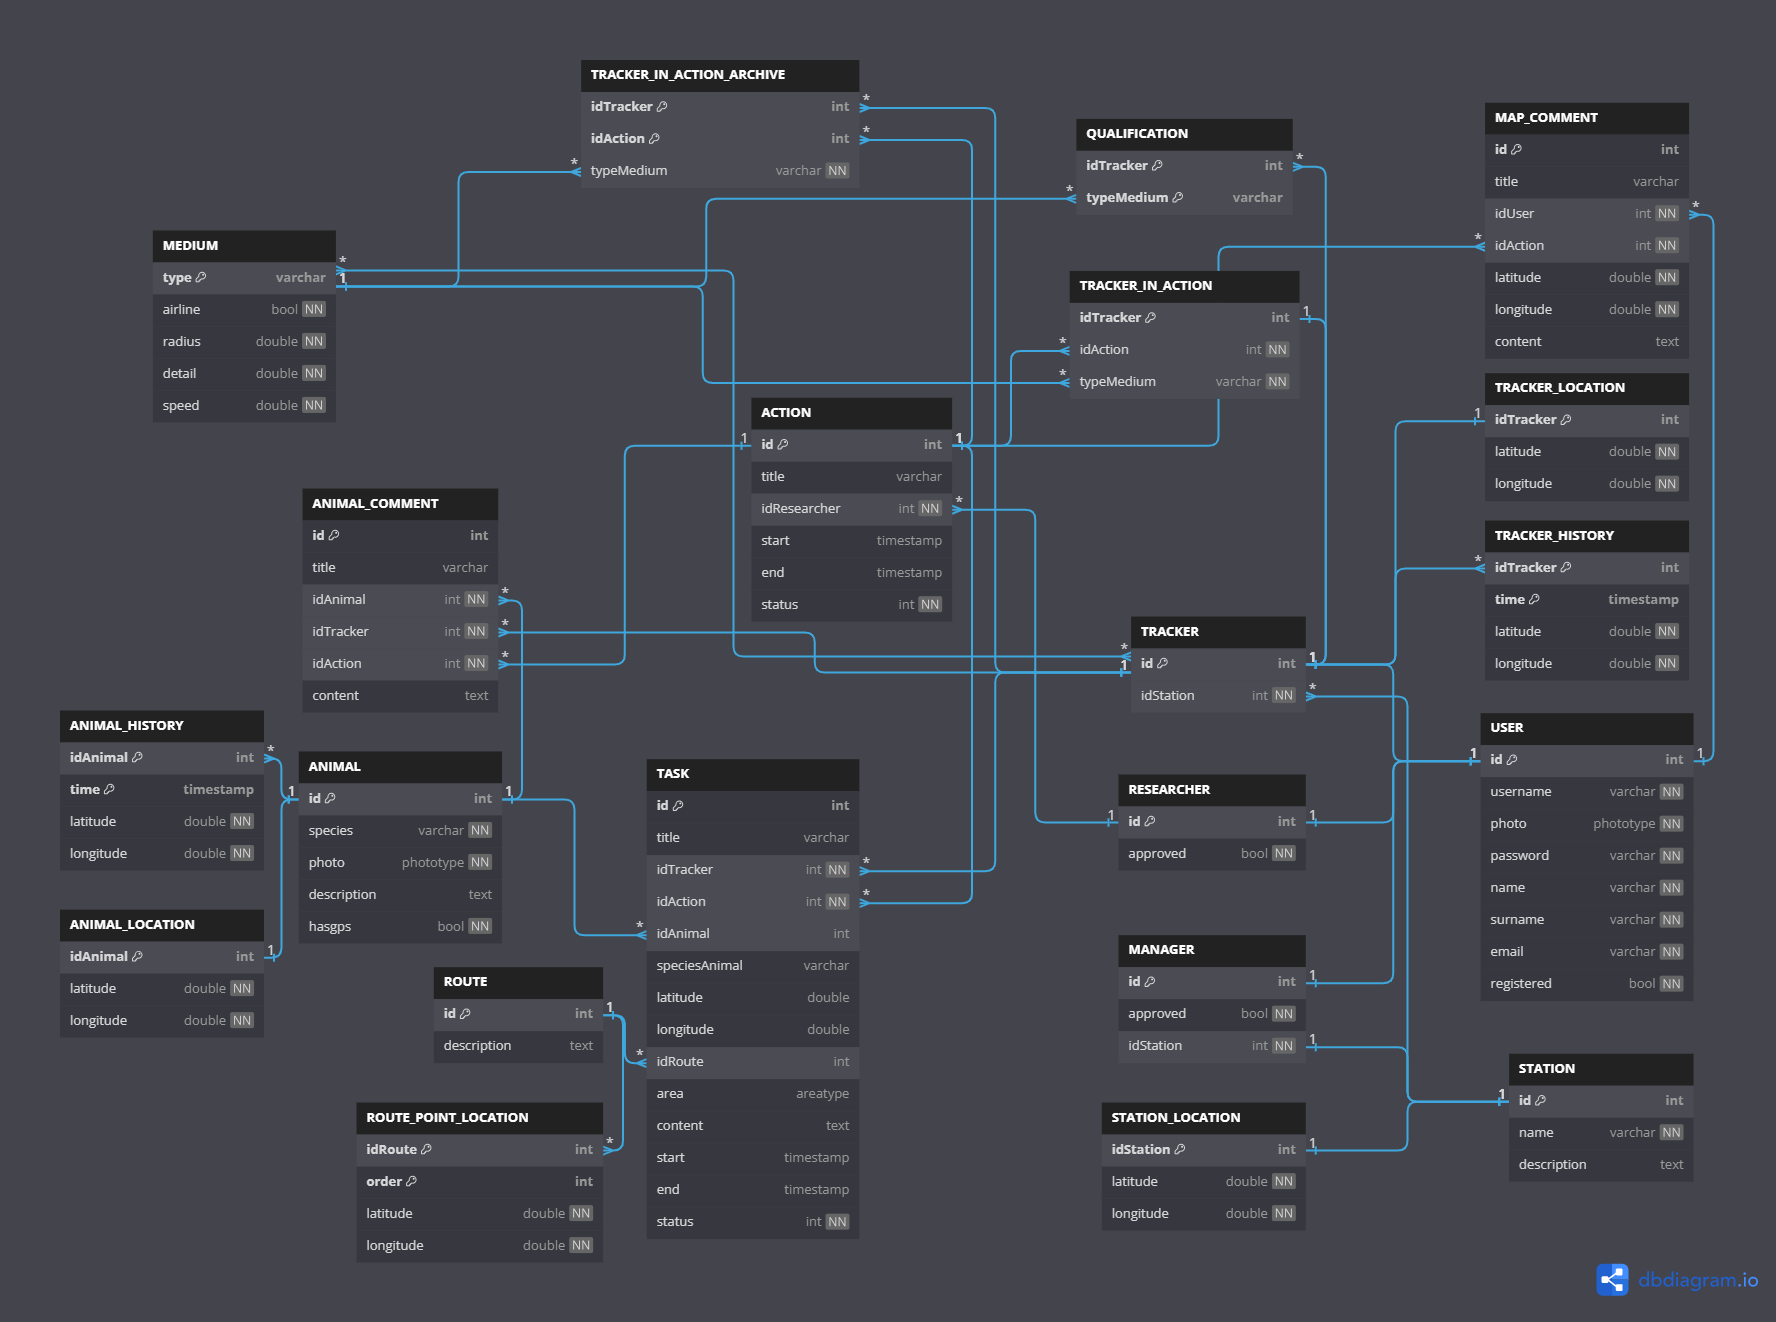
\includegraphics[scale=0.3]{slike/grafBaza.PNG} 
					% width=\textwidth,height=\textheight,keepaspectratio
					\centering
					\caption{E-R dijagram baze podataka}
					\label{fig:ERdiagram}
				\end{figure}				
				\restoregeometry
				
			\fi			
										
			
			\subsection{Dijagram baze podataka}			
			
				\vspace{12pt}						
				
				\begin{figure}[H] %ht
					\centering
					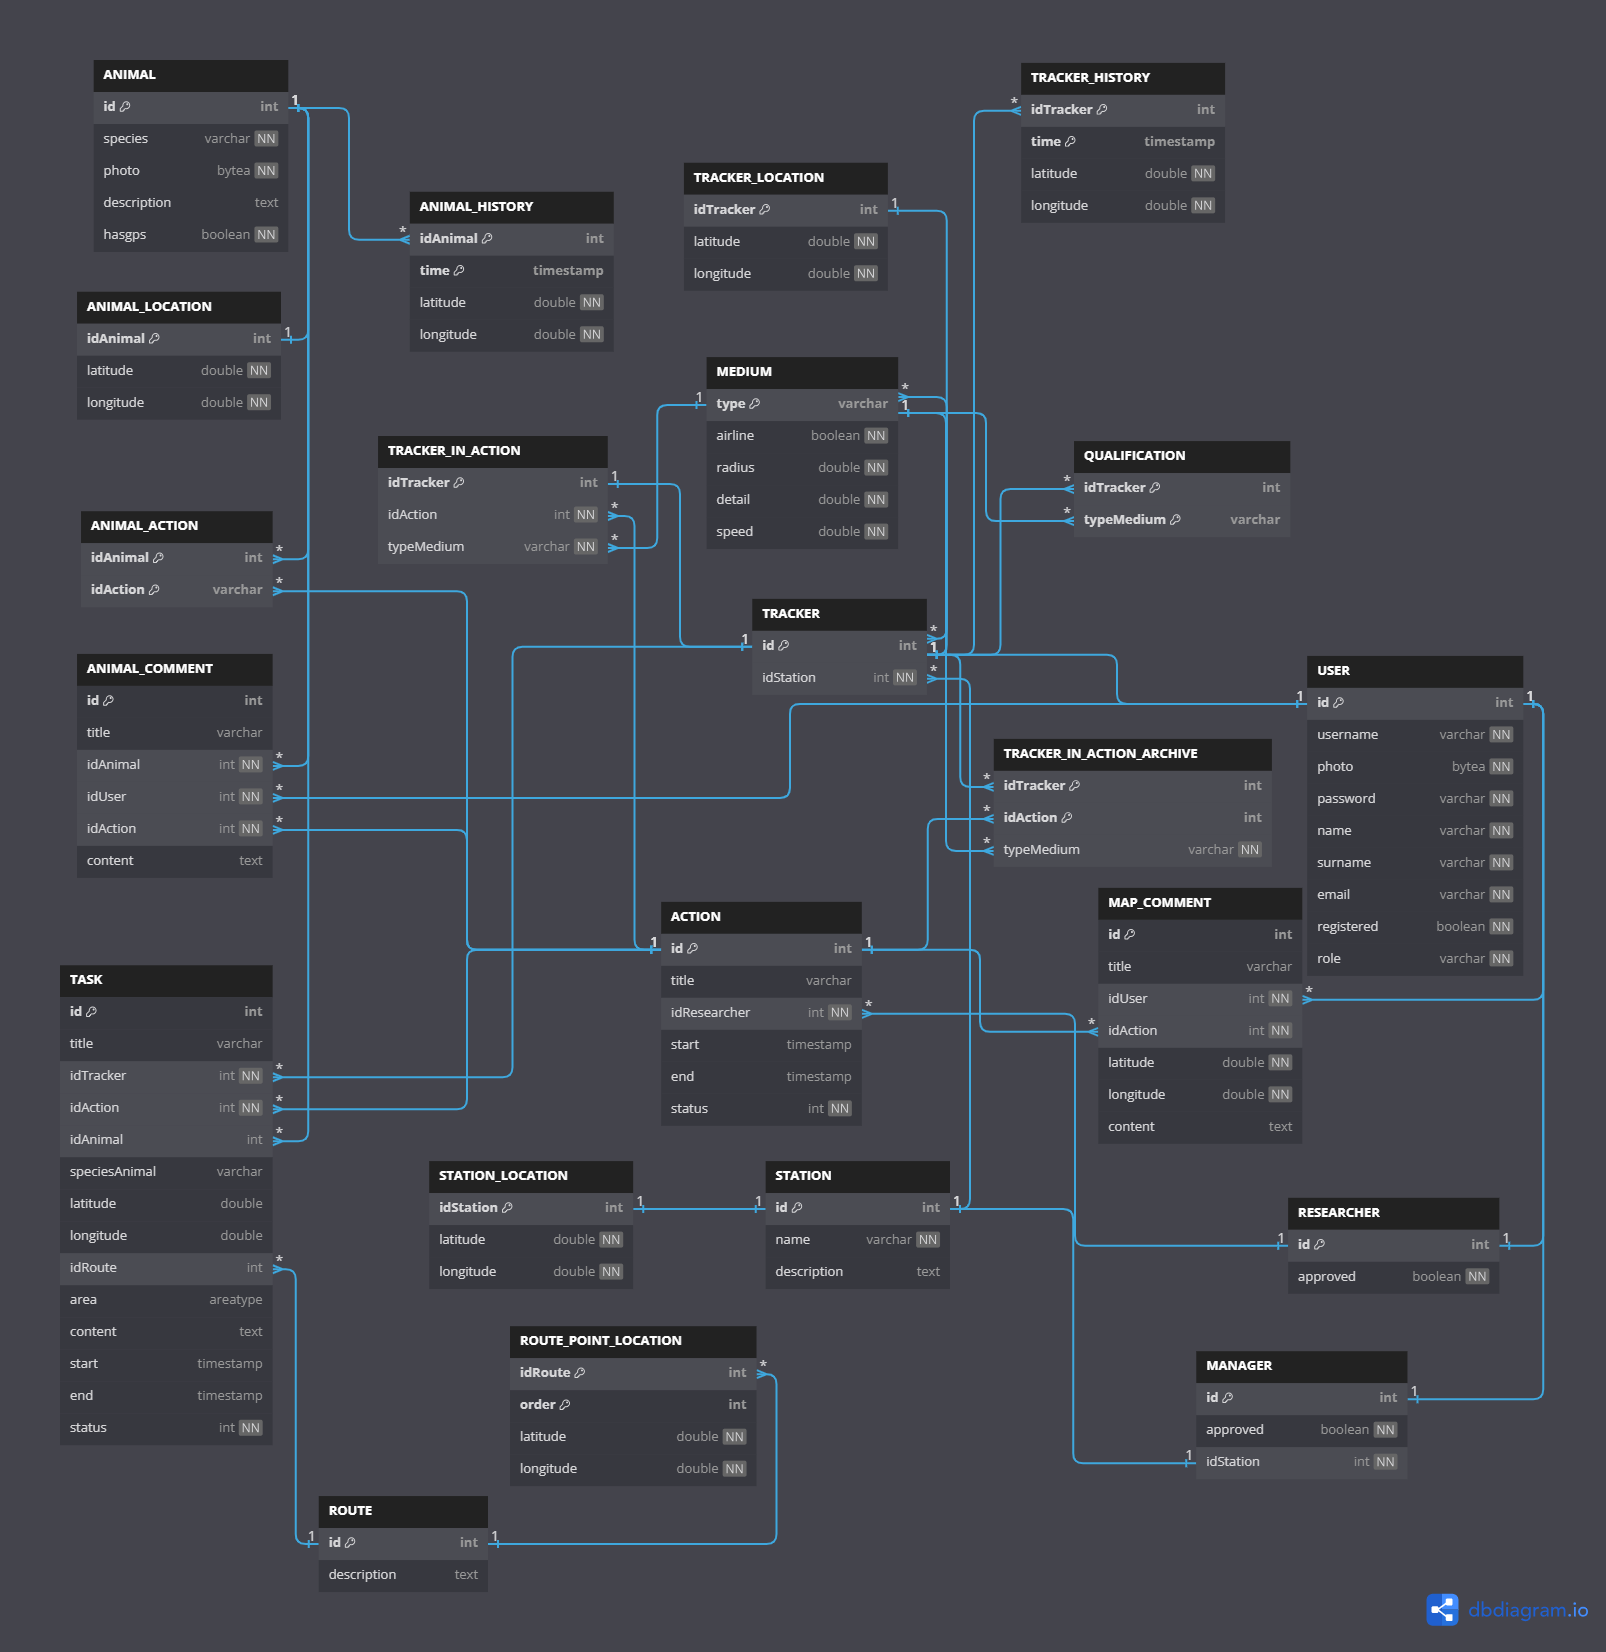
\includegraphics[width=\textwidth]{slike/baza.PNG}
					\caption{E-R dijagram baze podataka}
					\label{fig:ERdiagram}
				\end{figure}																												
																																	
			\eject
						
			
			
		\section{Dijagram razreda}
		
		\iffalse	\textit{Potrebno je priložiti dijagram razreda s pripadajućim opisom. Zbog preglednosti je moguće dijagram razlomiti na više njih, ali moraju biti grupirani prema sličnim razinama apstrakcije i srodnim funkcionalnostima.}\\
			
			\textbf{\textit{dio 1. revizije}}\\
			
			\textit{Prilikom prve predaje projekta, potrebno je priložiti potpuno razrađen dijagram razreda vezan uz \textbf{generičku funkcionalnost} sustava. Ostale funkcionalnosti trebaju biti idejno razrađene u dijagramu sa sljedećim komponentama: nazivi razreda, nazivi metoda i vrste pristupa metodama (npr. javni, zaštićeni), nazivi atributa razreda, veze i odnosi između razreda.}\\
			
			\textbf{\textit{dio 2. revizije}}\\			
			
			\textit{Prilikom druge predaje projekta dijagram razreda i opisi moraju odgovarati stvarnom stanju implementacije}
		\fi
			Na slikama 4.4, 4.5 i 4.6 prikazani su razredi koji pripadaju backend dijelu MVC arhitekture. Razredi prikazani na slici 4.3 nasljeđuju Controller razred. Metode implementirane u tim razredima obrađuju zahtjeve aktora koji dolaze s frontend servera obavljajući potrebne manipulacije podacima i šaljući odgovarajuće odgovore. Metode u Controller razredima obično vraćaju podatke u JSON formatu, a HTTP status kodovi koriste se za signalizaciju statusa zahtjeva (npr., uspješan odgovor, greška, itd.). Radi lakše organizacije, razredi su logički podijeljeni prema pravu pristupa metodama određenih aktera kako bi se smanjila prenapučenost unutar dijagrama. Prikazane su samo ovisnosti između razreda koji pripadaju istom dijelu dijagrama. Iz naziva i tipova atributa u razredima može se zaključiti vrsta ovisnosti među različitim razredima.Također se ponekad koriste dodatne DTO (Data transfer object) klase za specifične potrebe prijenosa podataka. Kod korištenja objekata koji predstavljaju modele ili DTO objekata u implementaciji selektivno se postavljaju atributi koji su potrebni za određene operacije, a ostali atributi su automatski postavljeni na null. To omogućuje modularno korištenje funkcija i zbog toga modeli i DTO objekti mogu imati reference na druge modele.
			
			\eject
		
			\vspace{12pt}						
			
			\begin{figure}[H] %ht
				\centering
				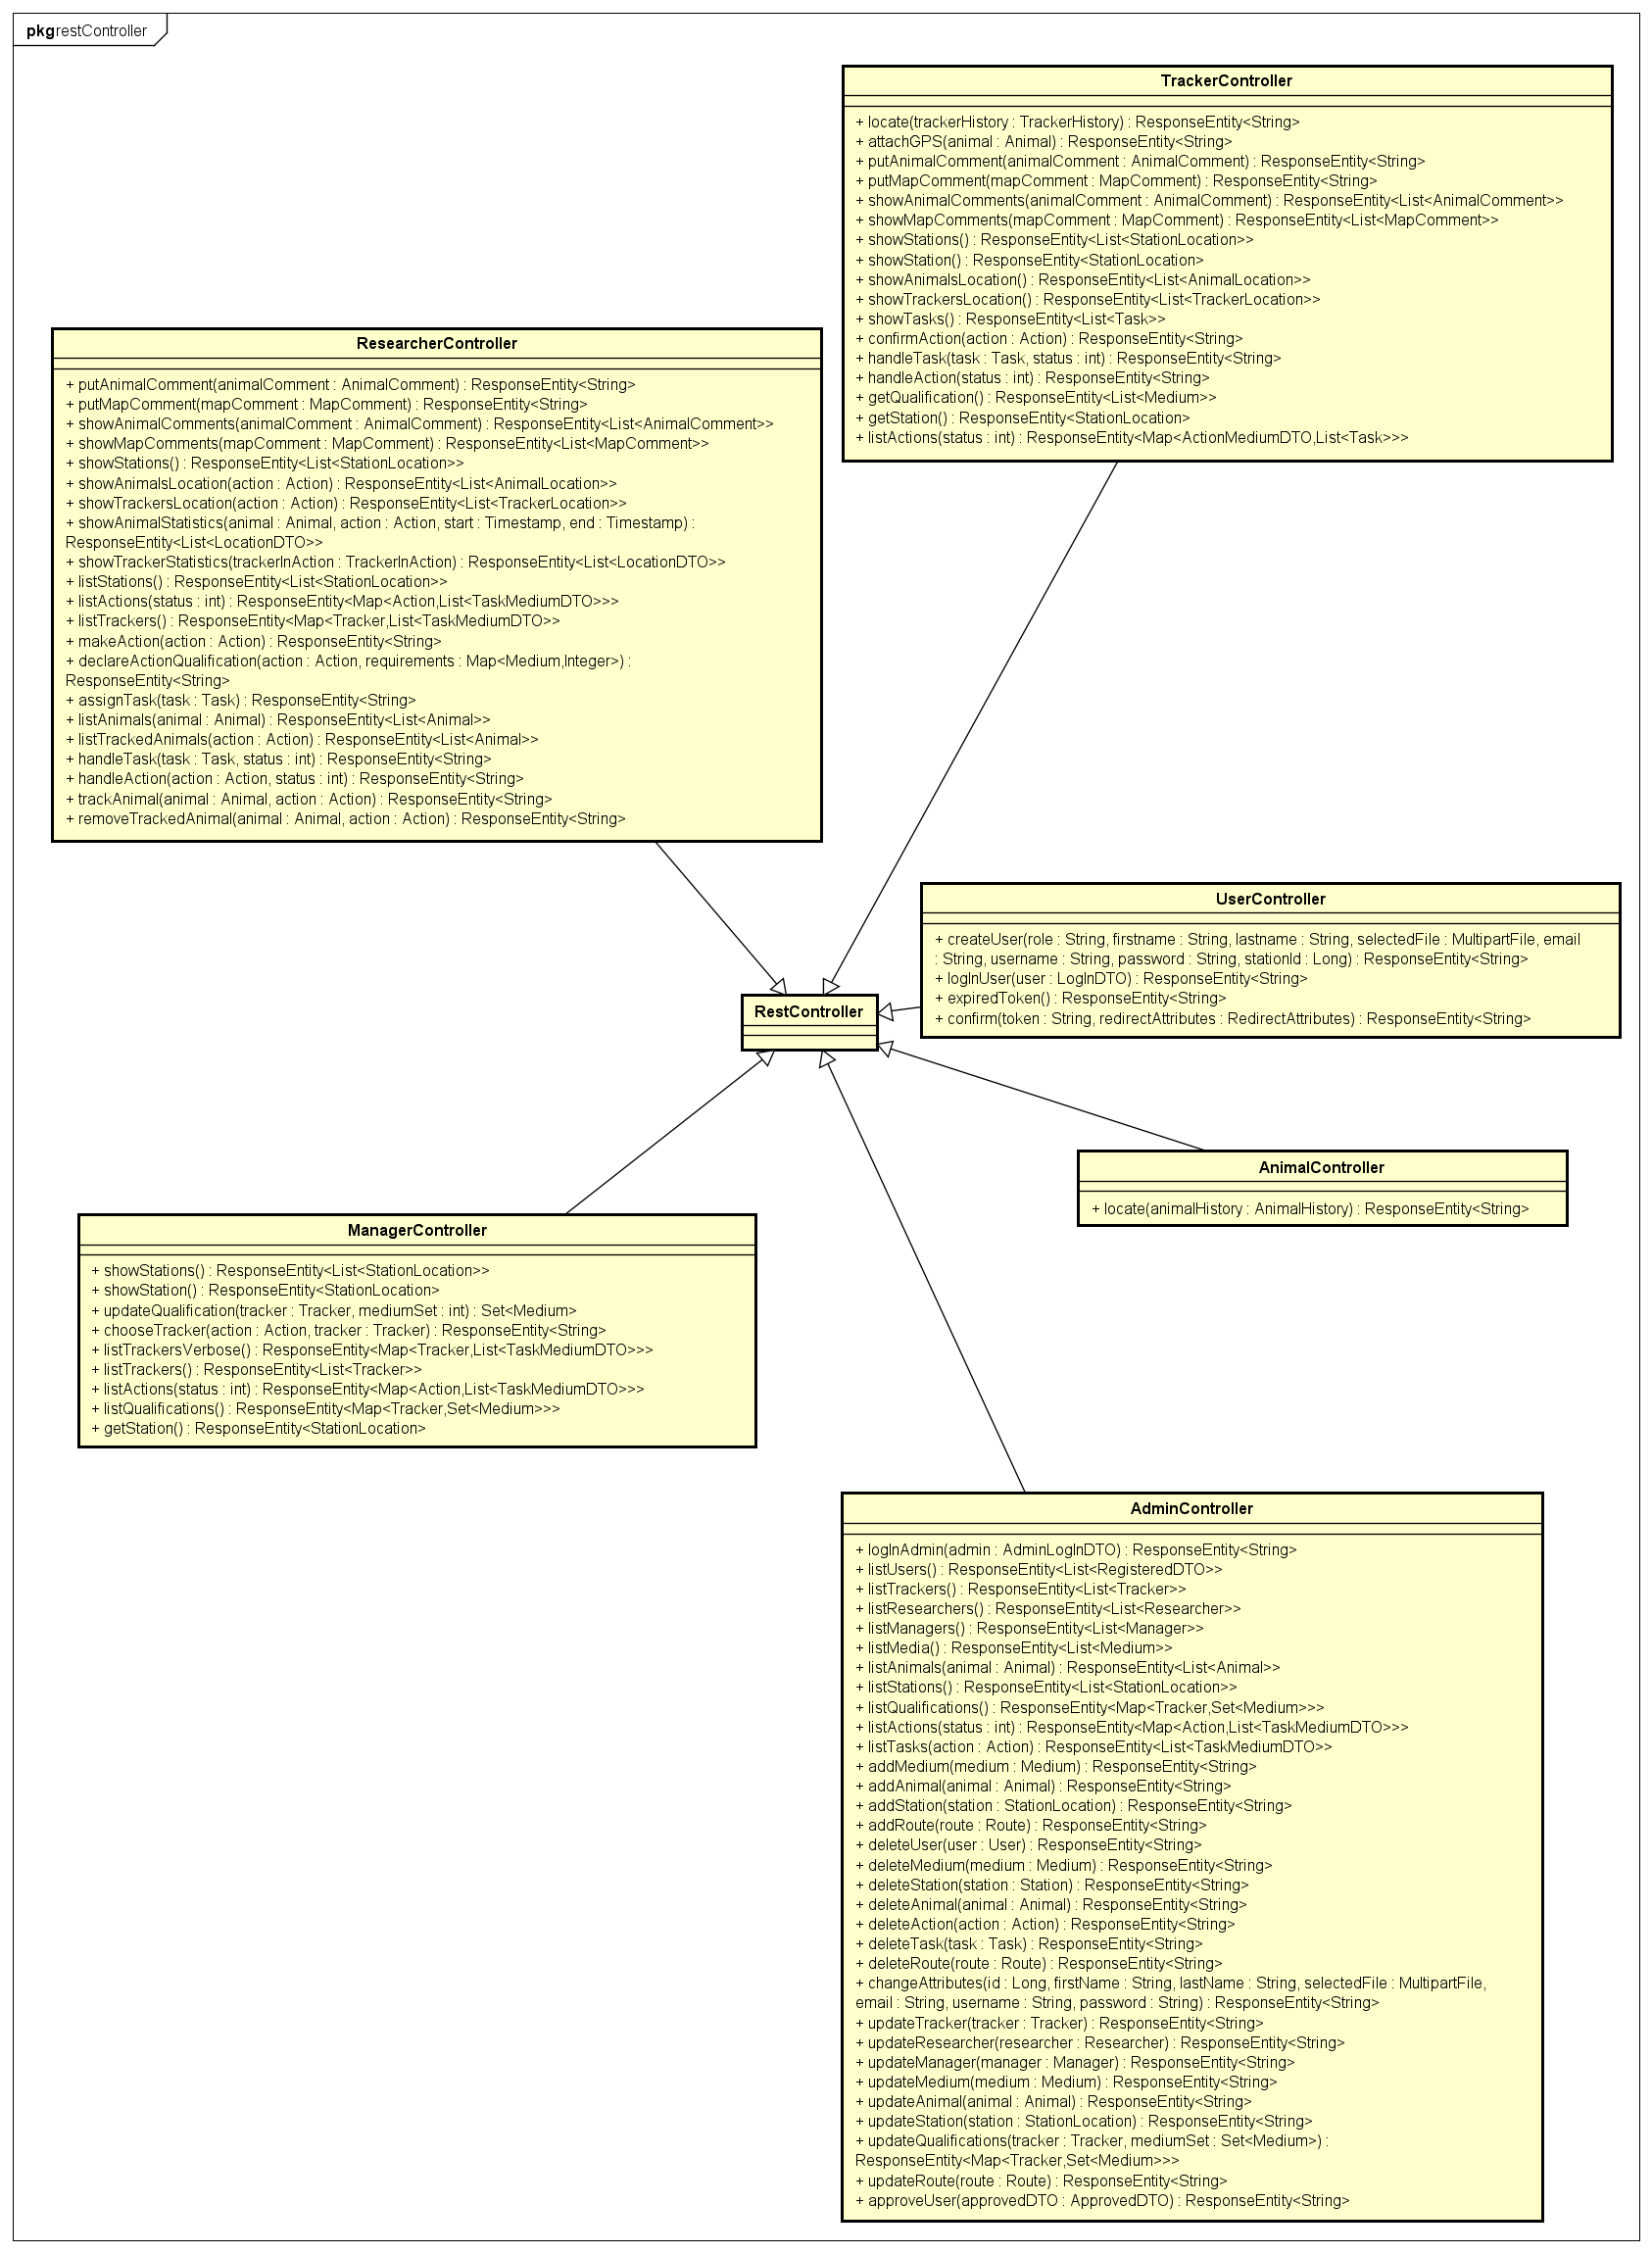
\includegraphics[width=\textwidth]{slike/controllerdiagram.png}
				\caption{Dijagram razreda - dio Controllers}
				\label{fig:Controllerdiagram}
			\end{figure}	
		
		\eject
		
		\begin{figure}[H] %ht
			\centering
			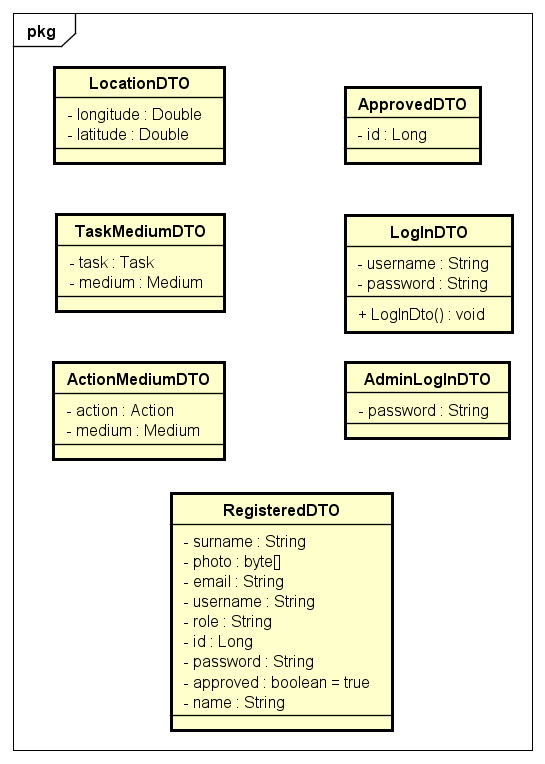
\includegraphics[width=\textwidth]{slike/dtodiagram.png}
			\caption{Dijagram razreda - dio Data transfer objects}
			\label{fig:DTOdiagram}
		\end{figure}
		
		\eject
		
		
		Model razredi preslikavaju strukturu baze podataka u aplikaciji. Svi entiteti realiziraju javne get i set metode za svoje privatne atribute. Modeli Researcher (istraživač), Tracker (tragač) i Manager (voditelj stanice) nasljeđuju model User (korisnik) te imaju svoje specifične atribute. Oni predstavljaju tri glavna tipa korisnika aplikacije od kojih svaki može upućivati specifične zahtjeve koji odražavaju mogućnosti tog tipa korisnika. Svaki korisnk se mora registrirati da bi koristio aplikaciju te korisnike tipa Researcher i Manager  administrator mora dodatno potvrditi. Istraživači organiziraju akcije s ciljem praćenja i prikupljanja podataka o životinjama, a na tim akcijama zadatke koje zadaje istraživač odrađuju tragači koji rade na toj akciji i pripadaju određenoj stanici koja ima svog voditelja koji odabire koji će tragači sudjelovati u nekoj akciji na temelju zahtjeva istraživača i kvalifikacija tragača. 
		
		\eject
		
		\begin{figure}[H] %ht
			\centering
			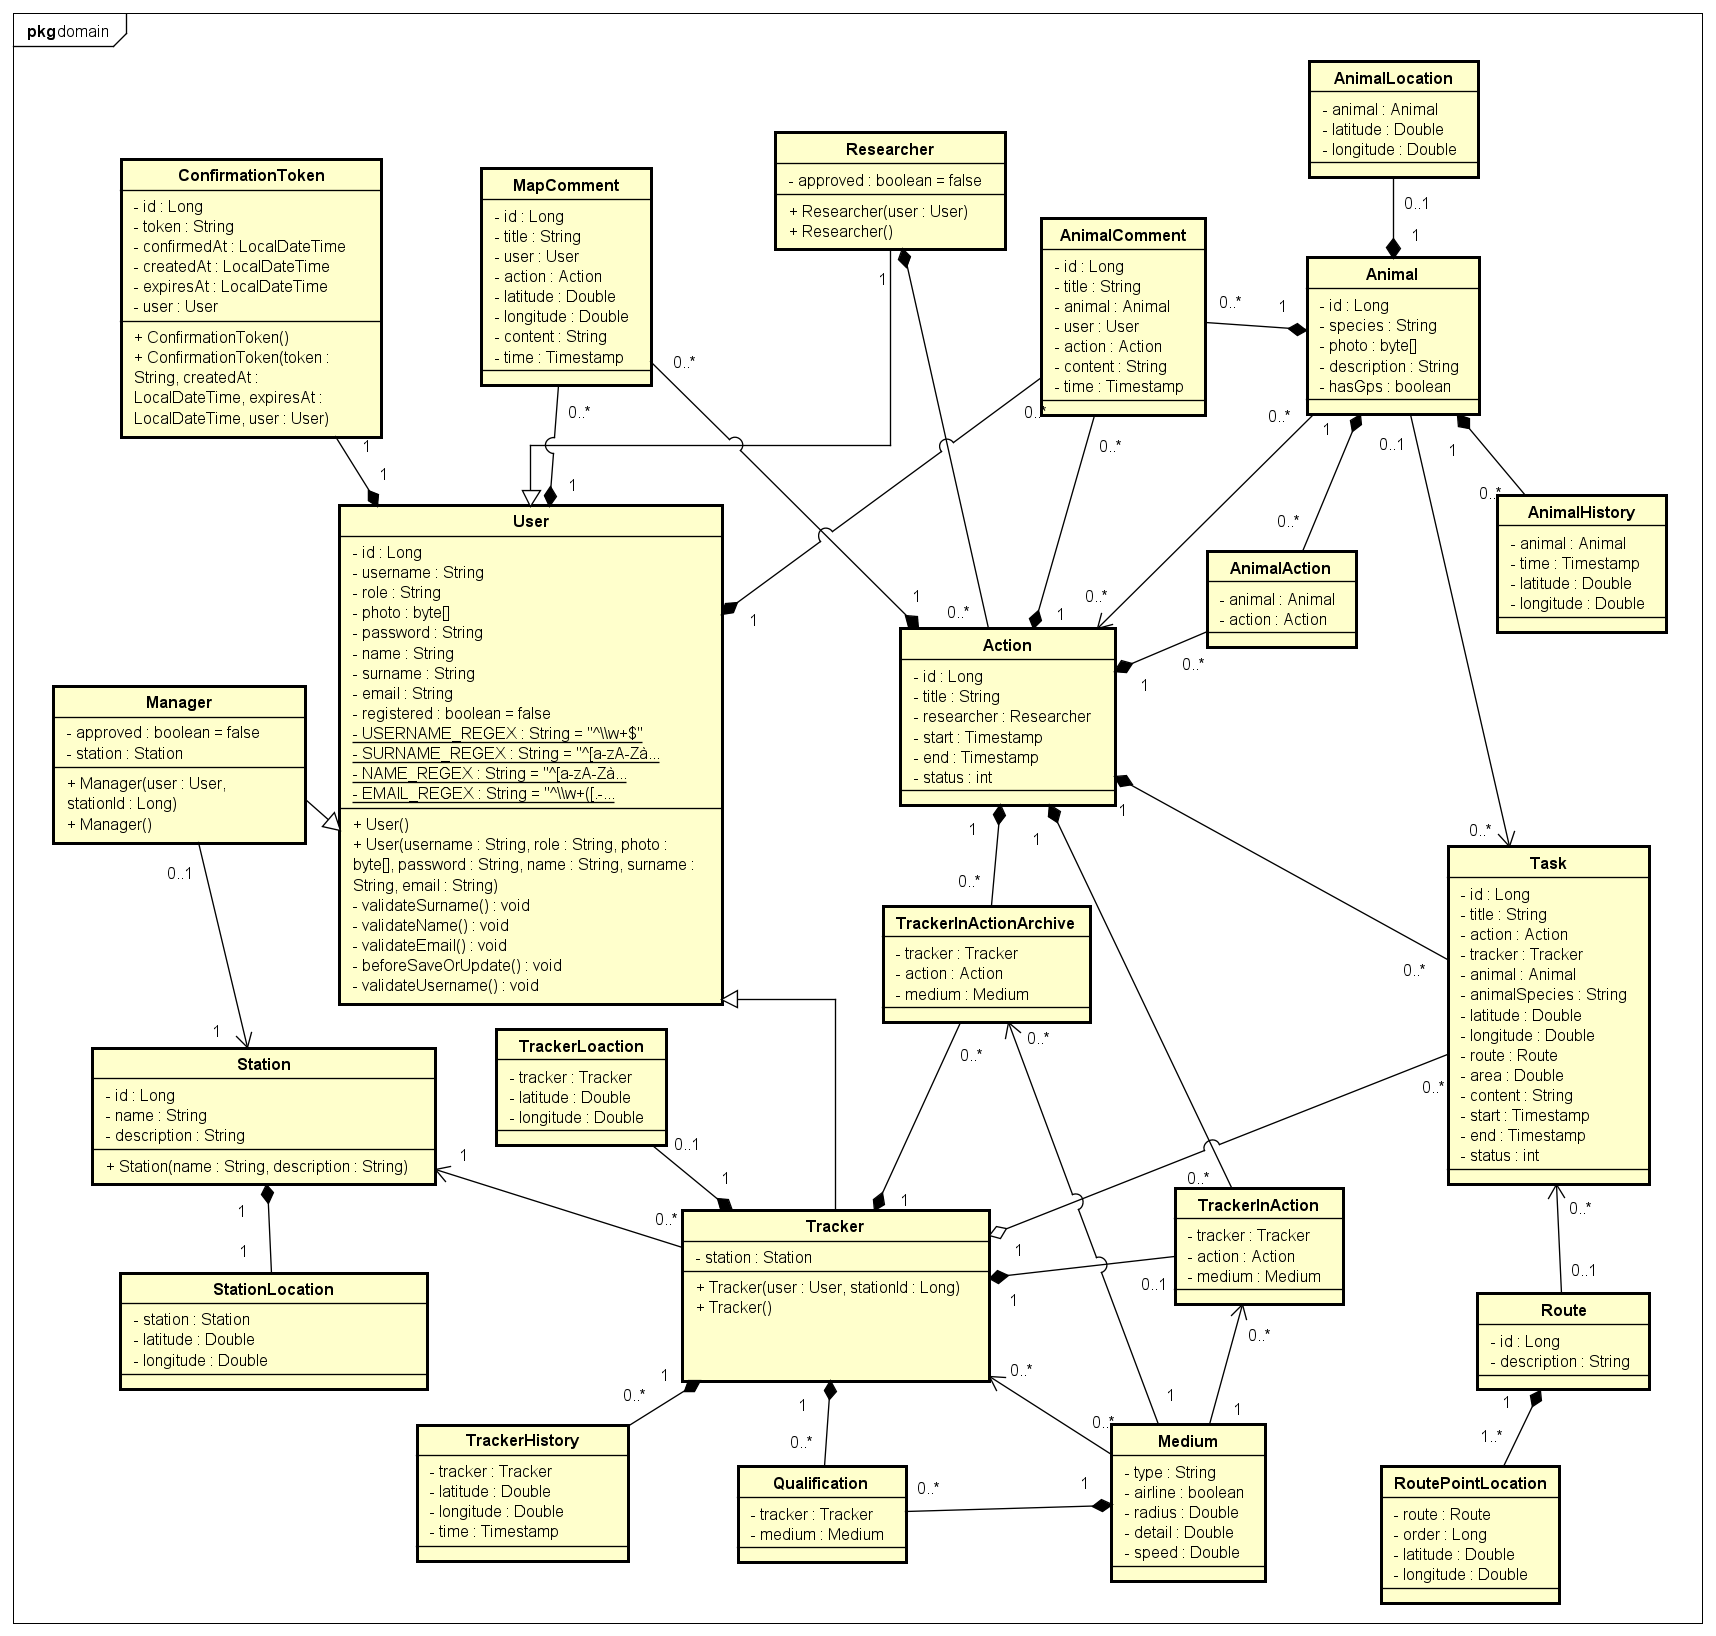
\includegraphics[width=\textwidth]{slike/modeldiagram.png}
			\caption{Dijagram razreda - dio Models}
			\label{fig:Modelrdiagram}
		\end{figure}
		
		\eject
		
		\section{Dijagram stanja}
			
			
			\noindent Dijagram stanja opisuje dinamičko ponašanje dijela sustava i prikazuje stanja objekata. Na slici ispod(slika 4.7) prikazuje se dijagram stanja za korisnika registriranog i ulogiranog kao Istraživač(Researcher).  Istraživaču se pokazuje početna stranica gdje ima mogućnost odabira 3 opcije: prikaza akcije, slanja zahtjeva za tragača i kreiranja nove akcije. Pri prikazu akcije istraživač može pogledati životinje koje se traže u akciji i može pogledati koji tragači su aktivni u akciji. Istraživač može popuniti zahtjev za tragača koji mu je potreban u akcijama i poslati ga na uvid voditelju. Novu akciju istraživač dodaje tako da klikne na dugme „create actions“, odabere tip akcije, odabere zadatke za svakog tragača i na kraju kreira akciju. Istraživač se može odjaviti u svakom trenutku.
			
			\begin{figure}[H]
				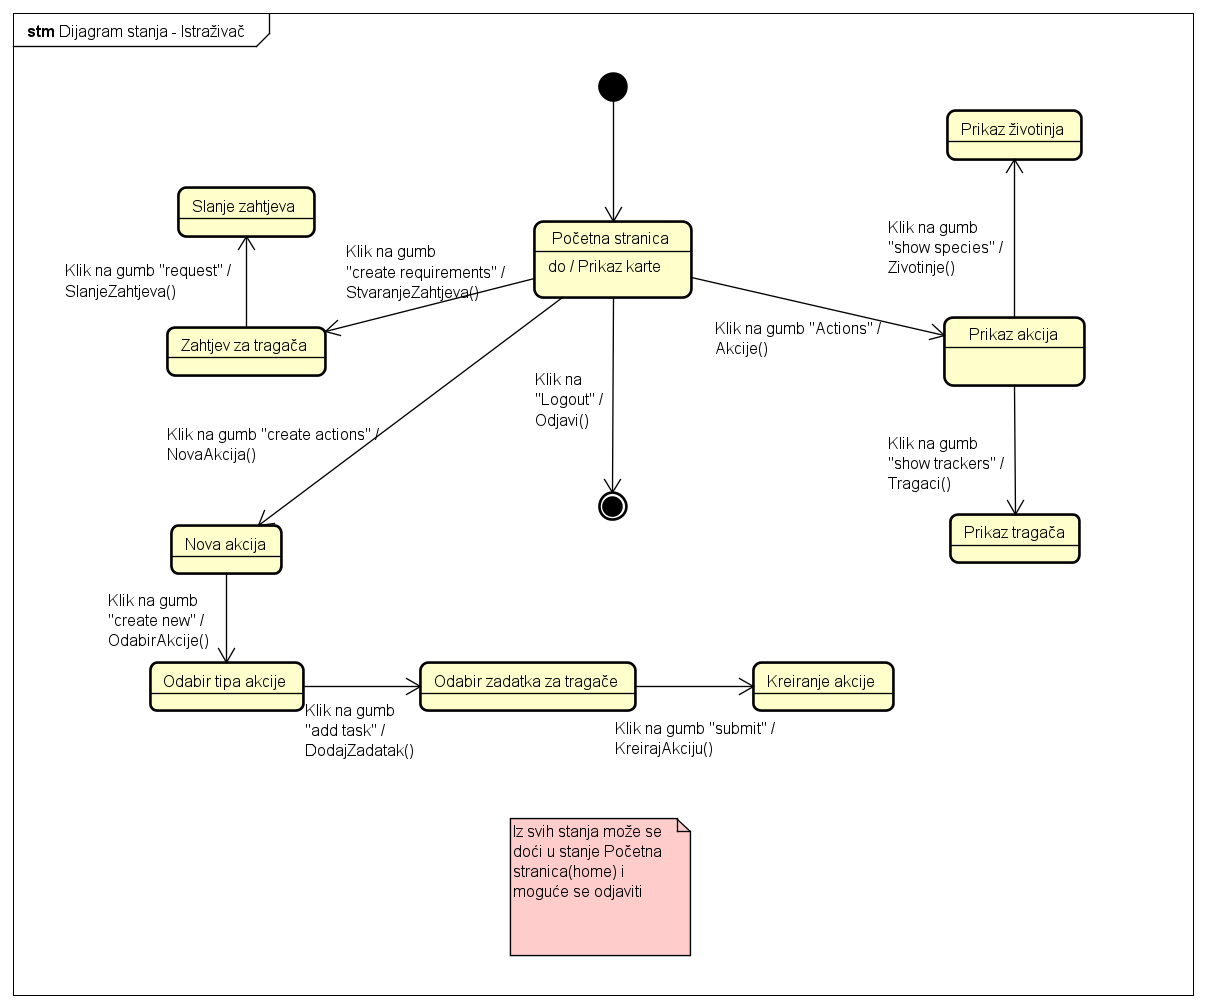
\includegraphics[scale=0.5]{slike/dijagram_stanja.PNG} %veličina slike u odnosu na originalnu datoteku i pozicija slike
				\centering
				\caption{Dijagram stanja}
				\label{fig:promjene}
			\end{figure}
			
			\eject 
		
		\section{Dijagram aktivnosti}
			
			\noindent Dijagram aktivnosti koristi se za opis modela toka upravljanja. Svaki korak u dijagramu odvija se nakon prethodno završenog te je dijagram vrlo čitljiv i lako razumljiv. Na slici ispod(slika 4.8) prikazan je dijagram aktivnosti za proces odabira podataka za prikazivanje na karti. Nakon što se korisnik prijavi u sustav, prikazuje mu se karta. Na njoj može odabrati opciju prikaza tragača ili opciju prikaza životinja. Aplikacija prikazuje željene podatke te korisnik nakon toga može odabrati prikaz toplinske karte i aplikacija mu to prikazuje.
			
			\begin{figure}[H]
				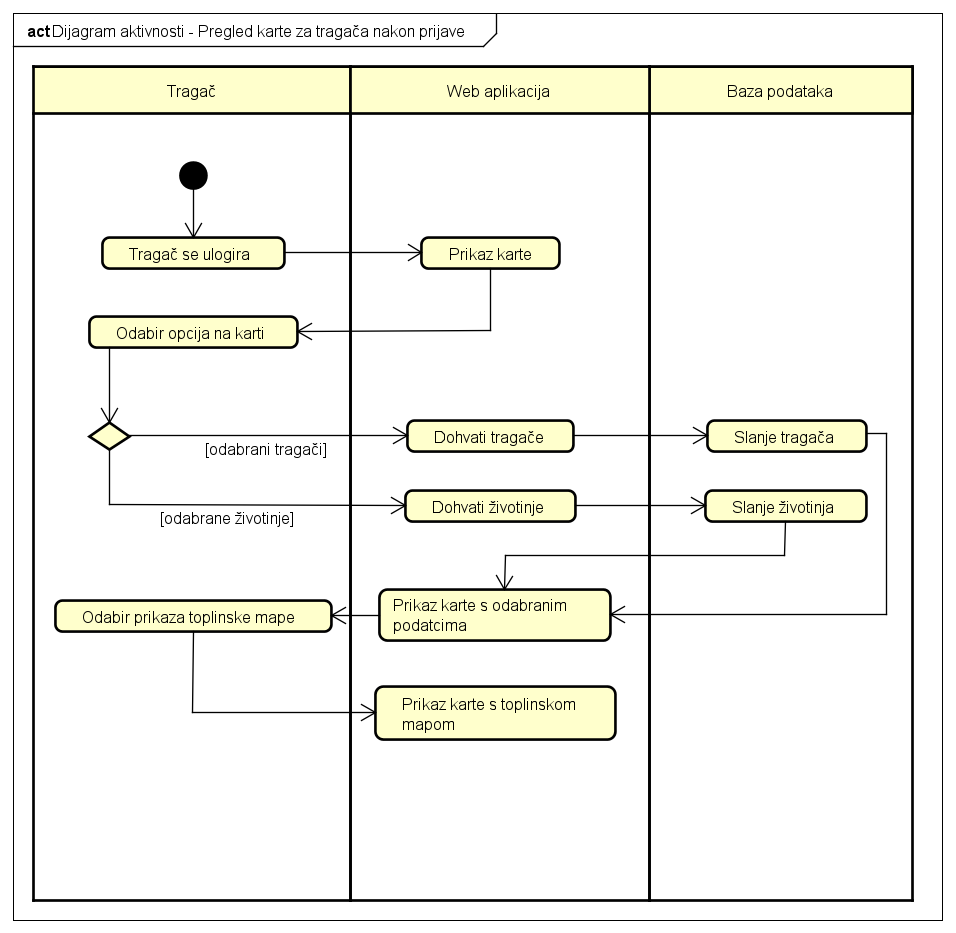
\includegraphics[scale=0.6]{slike/dijagram_aktivnosti.PNG} %veličina slike u odnosu na originalnu datoteku i pozicija slike
				\centering
				\caption{Dijagram aktivnosti}
				\label{fig:promjene}
			\end{figure}
			
			\eject
		\section{Dijagram komponenti}
		
			\noindent Dijagram komponenti opisuje organizaciju i međuovisnost komponenti, interne strukture i odnose prema okolini. Na slici ispod prikazan je dijagram sustava aplikacije WildTrack. Sustavu se pristupa preko dva sučelja. Pomoću sučelja za dohvat HTML, CSS i JS datoteka poslužuju se datoteke potrebne za frontend dio aplikacije. Pomoću router komponente, koja je dio Reacta, određuje se koje će se datoteke poslati na sučelje aplikacije.  Na frontendu se nalaze JavaScript datoteke koje zajedno čine razne komponente nazvane po aktorima kojima se pristupa. Preko sučelja za dohvat podataka u JSON obliku pristupa se REST API komponenti koja poslužuje podatke s backend dijela aplikacije. Hibernate komponenta dohvaća podatke iz SQL baze podataka te ih prosljeđuje DTO-u. Controller komponenta zadužena je primanje upita i odlučuje što se uzima od DTO komponente. React-view komponenta komunicira s aplikacijom i prikazuje potrebne podatke ovisno o zahtjevima.
			
			\begin{figure}[H]
				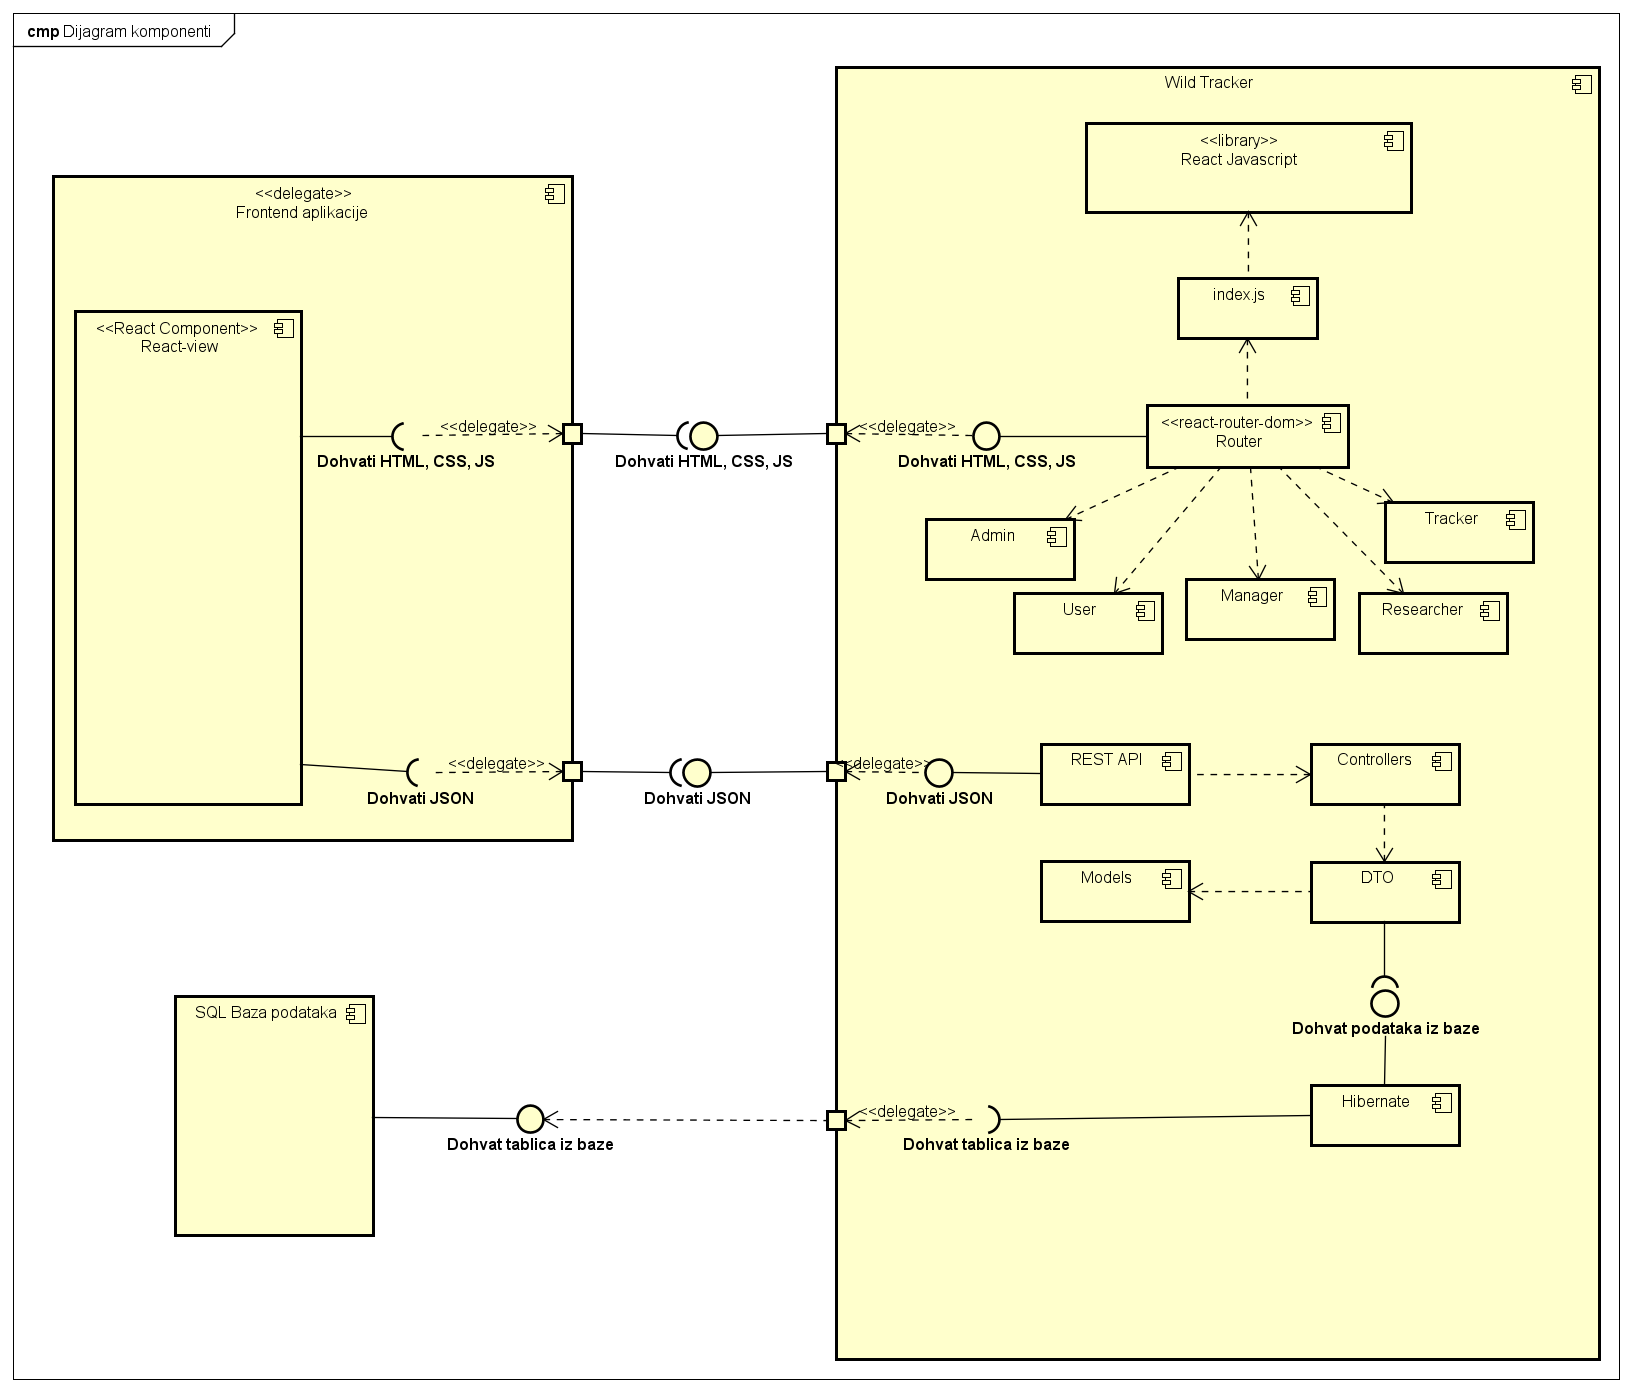
\includegraphics[scale=0.4]{slike/dijagram_komponenti.PNG} %veličina slike u odnosu na originalnu datoteku i pozicija slike
				\centering
				\caption{Dijagram komponenti}
				\label{fig:promjene}
			\end{figure}
	\chapter{Implementacija i korisničko sučelje}
		
		
		\section{Korištene tehnologije i alati}
		
			\textbf{\textit{dio 2. revizije}}
			
			 \textit{Detaljno navesti sve tehnologije i alate koji su primijenjeni pri izradi dokumentacije i aplikacije. Ukratko ih opisati, te navesti njihovo značenje i mjesto primjene. Za svaki navedeni alat i tehnologiju je potrebno \textbf{navesti internet poveznicu} gdje se mogu preuzeti ili više saznati o njima}.
			
			
			\eject 
		
	
		\section{Ispitivanje programskog rješenja}
			
			\textbf{\textit{dio 2. revizije}}\\
			
			 \textit{U ovom poglavlju je potrebno opisati provedbu ispitivanja implementiranih funkcionalnosti na razini komponenti i na razini cijelog sustava s prikazom odabranih ispitnih slučajeva. Studenti trebaju ispitati temeljnu funkcionalnost i rubne uvjete.}
	
			
			\subsection{Ispitivanje komponenti}
			\textit{Potrebno je provesti ispitivanje jedinica (engl. unit testing) nad razredima koji implementiraju temeljne funkcionalnosti. Razraditi \textbf{minimalno 6 ispitnih slučajeva} u kojima će se ispitati redovni slučajevi, rubni uvjeti te izazivanje pogreške (engl. exception throwing). Poželjno je stvoriti i ispitni slučaj koji koristi funkcionalnosti koje nisu implementirane. Potrebno je priložiti izvorni kôd svih ispitnih slučajeva te prikaz rezultata izvođenja ispita u razvojnom okruženju (prolaz/pad ispita). }
			
			
			
			\subsection{Ispitivanje sustava}
			
			 \textit{Potrebno je provesti i opisati ispitivanje sustava koristeći radni okvir Selenium\footnote{\url{https://www.seleniumhq.org/}}. Razraditi \textbf{minimalno 4 ispitna slučaja} u kojima će se ispitati redovni slučajevi, rubni uvjeti te poziv funkcionalnosti koja nije implementirana/izaziva pogrešku kako bi se vidjelo na koji način sustav reagira kada nešto nije u potpunosti ostvareno. Ispitni slučaj se treba sastojati od ulaza (npr. korisničko ime i lozinka), očekivanog izlaza ili rezultata, koraka ispitivanja i dobivenog izlaza ili rezultata.\\ }
			 
			 \textit{Izradu ispitnih slučajeva pomoću radnog okvira Selenium moguće je provesti pomoću jednog od sljedeća dva alata:}
			 \begin{itemize}
			 	\item \textit{dodatak za preglednik \textbf{Selenium IDE} - snimanje korisnikovih akcija radi automatskog ponavljanja ispita	}
			 	\item \textit{\textbf{Selenium WebDriver} - podrška za pisanje ispita u jezicima Java, C\#, PHP koristeći posebno programsko sučelje.}
			 \end{itemize}
		 	\textit{Detalji o korištenju alata Selenium bit će prikazani na posebnom predavanju tijekom semestra.}
			
			\eject 
		
		
		\section{Dijagram razmještaja}
			
			\textbf{\textit{dio 2. revizije}}
			
			 \textit{Potrebno je umetnuti \textbf{specifikacijski} dijagram razmještaja i opisati ga. Moguće je umjesto specifikacijskog dijagrama razmještaja umetnuti dijagram razmještaja instanci, pod uvjetom da taj dijagram bolje opisuje neki važniji dio sustava.}
			
			\eject 
		
		\section{Upute za puštanje u pogon}
		
			\textbf{\textit{dio 2. revizije}}\\
		
			 \textit{U ovom poglavlju potrebno je dati upute za puštanje u pogon (engl. deployment) ostvarene aplikacije. Na primjer, za web aplikacije, opisati postupak kojim se od izvornog kôda dolazi do potpuno postavljene baze podataka i poslužitelja koji odgovara na upite korisnika. Za mobilnu aplikaciju, postupak kojim se aplikacija izgradi, te postavi na neku od trgovina. Za stolnu (engl. desktop) aplikaciju, postupak kojim se aplikacija instalira na računalo. Ukoliko mobilne i stolne aplikacije komuniciraju s poslužiteljem i/ili bazom podataka, opisati i postupak njihovog postavljanja. Pri izradi uputa preporučuje se \textbf{naglasiti korake instalacije uporabom natuknica} te koristiti što je više moguće \textbf{slike ekrana} (engl. screenshots) kako bi upute bile jasne i jednostavne za slijediti.}
			
			
			 \textit{Dovršenu aplikaciju potrebno je pokrenuti na javno dostupnom poslužitelju. Studentima se preporuča korištenje neke od sljedećih besplatnih usluga: \href{https://aws.amazon.com/}{Amazon AWS}, \href{https://azure.microsoft.com/en-us/}{Microsoft Azure} ili \href{https://www.heroku.com/}{Heroku}. Mobilne aplikacije trebaju biti objavljene na F-Droid, Google Play ili Amazon App trgovini.}
			
			
			\eject 
	\part{title}\chapter{Zaključak i budući rad}
		
		\textbf{\textit{dio 2. revizije}}\\
		
		 \textit{U ovom poglavlju potrebno je napisati osvrt na vrijeme izrade projektnog zadatka, koji su tehnički izazovi prepoznati, jesu li riješeni ili kako bi mogli biti riješeni, koja su znanja stečena pri izradi projekta, koja bi znanja bila posebno potrebna za brže i kvalitetnije ostvarenje projekta i koje bi bile perspektive za nastavak rada u projektnoj grupi.}
		
		 \textit{Potrebno je točno popisati funkcionalnosti koje nisu implementirane u ostvarenoj aplikaciji.}
		
		\eject 
	\chapter*{Popis literature}
		\addcontentsline{toc}{chapter}{Popis literature}
	 	
 		\textbf{\textit{Kontinuirano osvježavanje}}
	
		\textit{Popisati sve reference i literaturu koja je pomogla pri ostvarivanju projekta.}
		
		
		\begin{enumerate}
			
			
			\item  Programsko inženjerstvo, FER ZEMRIS, \url{http://www.fer.hr/predmet/proinz}
			
			\item  I. Sommerville, "Software engineering", 8th ed, Addison Wesley, 2007.
			
			\item  T.C.Lethbridge, R.Langaniere, "Object-Oriented Software Engineering", 2nd ed. McGraw-Hill, 2005.
			
			\item  I. Marsic, Software engineering book``, Department of Electrical and Computer Engineering, Rutgers University, \url{http://www.ece.rutgers.edu/~marsic/books/SE}
			
			\item  The Unified Modeling Language, \url{https://www.uml-diagrams.org/}
			
			\item  Astah Community, \url{http://astah.net/editions/uml-new}
		\end{enumerate}
		
		 
	
	
	\begingroup
	\renewcommand*\listfigurename{Indeks slika i dijagrama}
	%\renewcommand*\listtablename{Indeks tablica}
	%\let\clearpage\relax
	\listoffigures
	%\vspace{10mm}
	%\listoftables
	\endgroup
	\addcontentsline{toc}{chapter}{Indeks slika i dijagrama}


	
	\eject 
		
	\chapter*{Dodatak: Prikaz aktivnosti grupe}
		\addcontentsline{toc}{chapter}{Dodatak: Prikaz aktivnosti grupe}
		
		\section*{Dnevnik sastajanja}
		
		
		\begin{packed_enum}
			\item  sastanak
			
			\item[] \begin{packed_item}
				\item Datum: 16. listopad 2023.
				\item Prisustvovali: M. S. Matušin, D. Baralić, L. Barišić, M. Bugarin, G. Oroz, N. Jamić, D. Štrbac
				\item Teme sastanka:
				\begin{packed_item}
					\item  upoznavanje
					\item  određivanje voditelja tima
				\end{packed_item}
			\end{packed_item}
			
			\item  sastanak
			\item[] \begin{packed_item}
				\item Datum: 20. listopad 2023.
				\item Prisustvovali: M. S. Matušin, D. Baralić, L. Barišić, M. Bugarin, G. Oroz, N. Jamić, D. Štrbac
				\item Teme sastanka:
				\begin{packed_item}
					\item  sastanak s asistentom
					\item  analiza zadatka
				\end{packed_item}
			\end{packed_item}
			
			\item  sastanak
			\item[] \begin{packed_item}
				\item Datum: 23. listopad 2023.
				\item Prisustvovali: M. S. Matušin, D. Baralić, L. Barišić, M. Bugarin, G. Oroz, N. Jamić, D. Štrbac
				\item Teme sastanka:
				\begin{packed_item}
					\item  raspodjela posla
					\item  konačan odabir alata i tehnologija
					\item rad na dokumentaciji
				\end{packed_item}
			\end{packed_item}
			
			\item  sastanak
			\item[] \begin{packed_item}
				\item Datum: 27. listopad 2023.
				\item Prisustvovali: M. S. Matušin, D. Baralić, L. Barišić, M. Bugarin, G. Oroz, N. Jamić, D. Štrbac
				\item Teme sastanka:
				\begin{packed_item}
					\item  sastanak s asistentom
					\item  razrješavanje dilema u vezi dokumentacije
					\item daljnja rapodjela zadataka
				\end{packed_item}
			\end{packed_item}
			
			\item  sastanak
			\item[] \begin{packed_item}
				\item Datum: 3. studeni 2023.
				\item Prisustvovali: M. S. Matušin, N. Jamić
				\item Teme sastanka:
				\begin{packed_item}
					\item  rad na backendu aplikacije
				\end{packed_item}
			\end{packed_item}
			
			\item  sastanak
			\item[] \begin{packed_item}
				\item Datum: 7. studeni 2023.
				\item Prisustvovali: M. S. Matušin, D. Baralić, L. Barišić, M. Bugarin, G. Oroz, N. Jamić, D. Štrbac
				\item Teme sastanka:
				\begin{packed_item}
					\item  zajednički rad na aplikaciji
					\item  dogovaranje za dizajn stranice
					\item daljnja raspodjela zadataka
				\end{packed_item}
			\end{packed_item}
			
			\item  sastanak
			\item[] \begin{packed_item}
				\item Datum: 12. studeni 2023.
				\item Prisustvovali: M. S. Matušin, N. Jamić
				\item Teme sastanka:
				\begin{packed_item}
					\item  rad na backendu aplikacije
				\end{packed_item}
			\end{packed_item}
		
			
			%
			
		\end{packed_enum}
		
		\eject
		\section*{Tablica aktivnosti}
		
			\begin{longtblr}[
					label=none,
				]{
					vlines,hlines,
					width = \textwidth,
					colspec={X[7, l]X[1, c]X[1, c]X[1, c]X[1, c]X[1, c]X[1, c]X[1, c]}, 
					vline{1} = {1}{text=\clap{}},
					hline{1} = {1}{text=\clap{}},
					rowhead = 1,
				} 
			
				\SetCell[c=1]{c}{} & \SetCell[c=1]{c}{\rotatebox{90}{\textbf{Mia Sara Matušin}}} & \SetCell[c=1]{c}{\rotatebox{90}{\textbf{Dino Baralić }}} &	\SetCell[c=1]{c}{\rotatebox{90}{\textbf{Lana Barišić }}} & \SetCell[c=1]{c}{\rotatebox{90}{\textbf{Martin Bugarin }}} &	\SetCell[c=1]{c}{\rotatebox{90}{\textbf{Nikola Jamić }}} & \SetCell[c=1]{c}{\rotatebox{90}{\textbf{Gabriela Oroz }}} &	\SetCell[c=1]{c}{\rotatebox{90}{\textbf{Dorjan Štrbac }}} \\  
				Upravljanje projektom 		&5  &  &  &  &  &  & \\ 
				Opis projektnog zadatka 	&5  &  &  &  &  &  & \\ 
				
				Funkcionalni zahtjevi       &  &  &  &  &3  &  &  \\ 
				Opis pojedinih obrazaca 	&  &  &7  &  &  &5  &  \\ 
				Dijagram obrazaca 			&  &  &2  &  &  &  &  \\ 
				Sekvencijski dijagrami 		&  &  &  &4  &  &  &  \\ 
				Opis ostalih zahtjeva 		&  &  &  &1  &  &  &  \\ 

				Arhitektura i dizajn sustava	 &  &  &3  &  &  &  &  \\ 
				Baza podataka				&  &10  &  &  &  &  &10   \\ 
				Dijagram razreda 			&  &12  &  &  &  &  &12   \\ 
				Dijagram stanja				&  &  &  &  &  &  &  \\ 
				Dijagram aktivnosti 		&  &  &  &  &  &  &  \\ 
				Dijagram komponenti			&  &  &  &  &  &  &  \\ 
				Korištene tehnologije i alati 		&  &  &  &  &  &  &  \\ 
				Ispitivanje programskog rješenja 	&  &  &  &  &  &  &  \\ 
				Dijagram razmještaja			&  &  &  &  &  &  &  \\ 
				Upute za puštanje u pogon 		&  &  &  &  &  &  &  \\  
				Dnevnik sastajanja 			&1  &  &  &  &  &  &  \\ 
				Zaključak i budući rad 		&  &  &  &  &  &  &  \\  
				Popis literature 			&1  &  &  &  &  &  &  \\  
				\hline
				Front end 				&  &  &20  &21  &  &20  &  \\  
				Back end 							&30  &  &  &  &30  &  &10  \\  
			\end{longtblr}
					
					
		\eject
		\section*{Dijagrami pregleda promjena}
		
		\textbf{\textit{dio 2. revizije}}\\
		
		\textit{Prenijeti dijagram pregleda promjena nad datotekama projekta. Potrebno je na kraju projekta generirane grafove s gitlaba prenijeti u ovo poglavlje dokumentacije. Dijagrami za vlastiti projekt se mogu preuzeti s gitlab.com stranice, u izborniku Repository, pritiskom na stavku Contributors.}
		
	


\end{document} %naredbe i tekst nakon ove naredbe ne ulaze u izgrađen dokument 


